%% This is a sample manuscript marked up using the
%% AASTeX v5.x LaTeX 2e macros.

%% The first piece of markup in an AASTeX v5.x document
%% is the \documentclass command. LaTeX will ignore
%% any data that comes before this command.

%% The command below calls the preprint style
%% which will produce a one-column, single-spaced document.
%% Examples of commands for other substyles follow. Use
%% whichever is most appropriate for your purposes.
%%

%\documentclass[11pt,preprint2]{aastex}
% manuscript produces a one-column, double-spaced document:
%\documentclass[manuscript]{aastex}
%% preprint2 produces a double-column, single-spaced document:

%\documentclass{emulateapj}
\documentclass[preprint]{aastex}

\usepackage{natbib}
\usepackage{amsmath}
\bibliographystyle{apj}
\usepackage{graphicx}

%% Sometimes a paper's abstract is too long to fit on the
%% title page in preprint2 mode. When that is the case,
%% use the longabstract style option.

%% \documentclass[preprint2,longabstract]{aastex}

%% If you want to create your own macros, you can do so
%% using \newcommand. Your macros should appear before
%% the \begin{document} command.
%%
%% If you are submitting to a journal that translates manuscripts
%% into SGML, you need to follow certain guidelines when preparing
%% your macros. See the AASTeX v5.x Author Guide
%% for information.

%% You can insert a short comment on the title page using the command below.

%\slugcomment{Not to appear in Nonlearned J., 45.}

%% If you wish, you may supply running head information, although
%% this information may be modified by the editorial offices.
%% The left head contains a list of authors,
%% usually a maximum of three (otherwise use et al.).  The right
%% head is a modified title of up to roughly 44 characters.
%% Running heads will not print in the manuscript style.

%\shorttitle{HERA Dish Beam Measurements Memo, Rev $\alpha$}
%\shortauthors{Neben}

%% This is the end of the preamble.  Indicate the beginning of the
%% paper itself with \begin{document}.

\begin{document}

\title{HERA Dish Beam Measurements Memo, Rev. $\alpha$}

%% Use \author, \affil, and the \and command to format
%% author and affiliation information.
%% Note that \email has replaced the old \authoremail command
%% from AASTeX v4.0. You can use \email to mark an email address
%% anywhere in the paper, not just in the front matter.
%% As in the title, use \\ to force line breaks.

\author{Abraham Neben, Rich Bradley, Jackie Hewitt}
%\affil{MIT Kavli Institute, Massachusetts Institute of Technology, Cambridge, MA, 02139 USA}

\author{Oct 25, 2015}
%\affil{Wasamatta U}

%% Notice that each of these authors has alternate affiliations, which
%% are identified by the \altaffilmark after each name.  Specify alternate
%% affiliation information with \altaffiltext, with one command per each
%% affiliation.

%% Mark off your abstract in the ``abstract'' environment. In the manuscript
%% style, abstract will output a Received/Accepted line after the
%% title and affiliation information. No date will appear since the author
%% does not have this information. The dates will be filled in by the
%% editorial office after submission.

\begin{abstract}
write abstract here
comment on how this expt is still a work in progress
\end{abstract}

%\keywords{instrumentation: interferometers --- techniques: interferometric --- cosmology: observations --- dark ages, reionization, first stars}

%\section{Other title ideas}
%\begin{itemize}
%\item The relationship between noise correlation and monopole sensitivity in radio interferometers
%\item The self noise of sky noise in monopole interferometers
%\item Signal and noise in global signal interferometers
%\end{itemize}



%\section{Introduction}

\section{Experimental Setup}

We review the 


\begin{figure*}[h]
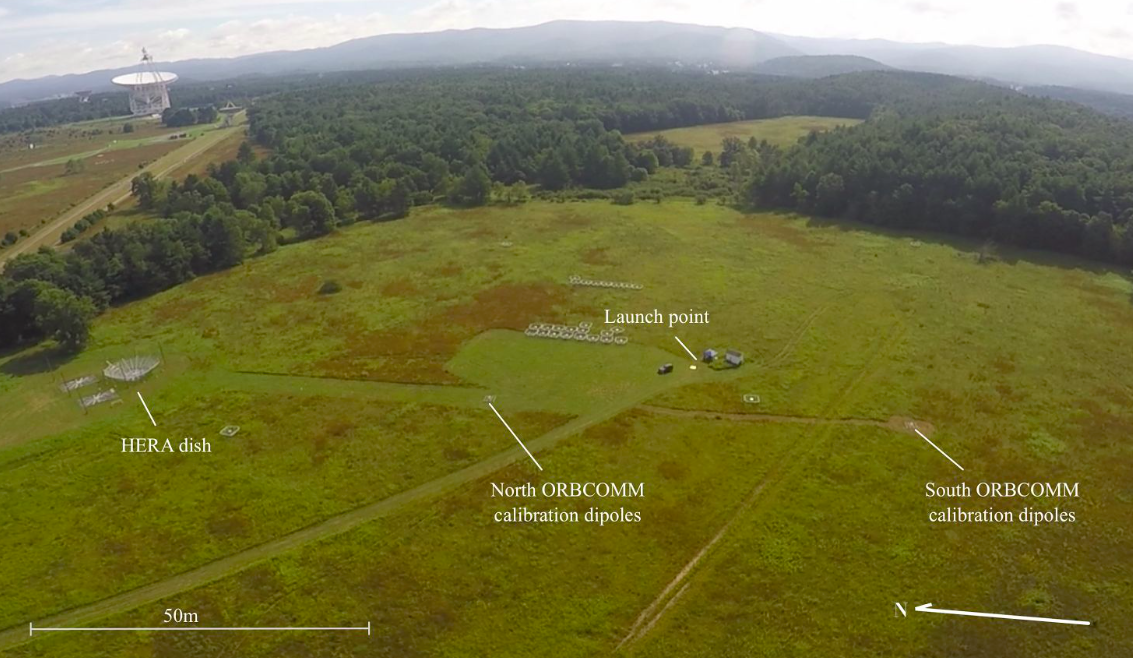
\includegraphics[width=6.5in]{aerial.png}
\caption{Aerial photograph of the two reference dipoles deployed in Galford Meadow at the National Radio Astronomy Observatory--Green Bank 100\,m south of the HERA dish.}
\label{fig:null3}
\end{figure*}


specify which of the three HERA dishes we are talking about 

sky coverage with orbcomm experiment

\section{Beam Modeling}

\subsection{Reference antenna model}
Our power ratio measurement relies upon an accurately modeled reference dipole, and to that end we improve on the model used in \citep{neben15} by XXX

\subsection{Dish models}
\label{sec:dishmodels}

We compare measured beam patterns with a simplistic analytic model and two numerical electromagnetic models. NEED MORE DETAILS ABOUT MODELING
\begin{enumerate}
	\item Airy pattern for a 14\,m aperture
	\item CST simulation (\texttt{hera-cst/HERA\_DISH\_paper\_feed\_cyl36\_140mhz\_Y\_healpix.fits})
	\item A separate simulation run by Dave
\end{enumerate}

\section{Null Experiments}

As in \citet{neben15}, we assess systematics using a ``null experiment'' in which we use a second reference dipole as the antenna-under-test (AUT). Taking the ratio of its measured power pattern with the model beam pattern amounts to a ratio of the row power responses received by the two antennas. This test thus probes the level of environmental systematics (i.e., reflections and varying ground properties) and antenna fabrication imperfections which affect each antenna differently. This is not a probe of modeling imperfections common to both antennas, but we expect such errors to be subdominant as the physical properties of the antenna are easier to characterize, and thus simulate, than local environmental effects. 

We run three null experiments with the reference dipoles deployed varying distances from the HERA dish and from each other.

\begin{itemize}
\item \texttt{null1}: reference dipoles deployed 50\,m apart on a NS line, 50\,m south of the HERA dish
\item \texttt{null3}: same as \texttt{null1} but with the south-most reference antenna moved 5\,m west
\item \texttt{null4}: same as \texttt{null1} but with 100\,m separation between both reference antennas and from the dish
\end{itemize}

Figure \ref{fig:null1} shows the results from the \texttt{null1} experiment in the form of the ratio of the power responses of the two antennas (top panel), and slices through the E an H planes of the reconstructed power patterns (bottom panel). We collected roughly 100 satellite passes. Systematics at the few percent level are observed in  within $20^\circ$ of zenith, and at the $\sim10\%$ level farther out.

The magnitude of these systematics is comparable to those observed in the two other null experiments (Figures \ref{fig:null3} and \ref{fig:null4}), an their angular distribution appears largely unchanged. This suggests that the reference dipoles differ both due to varying environmental properties and perhaps intrinsic differences. In any case, these fractional errors propagate directly into the measured beampatterns of our subsequent feed and dish measurements.  

\begin{figure*}[h]
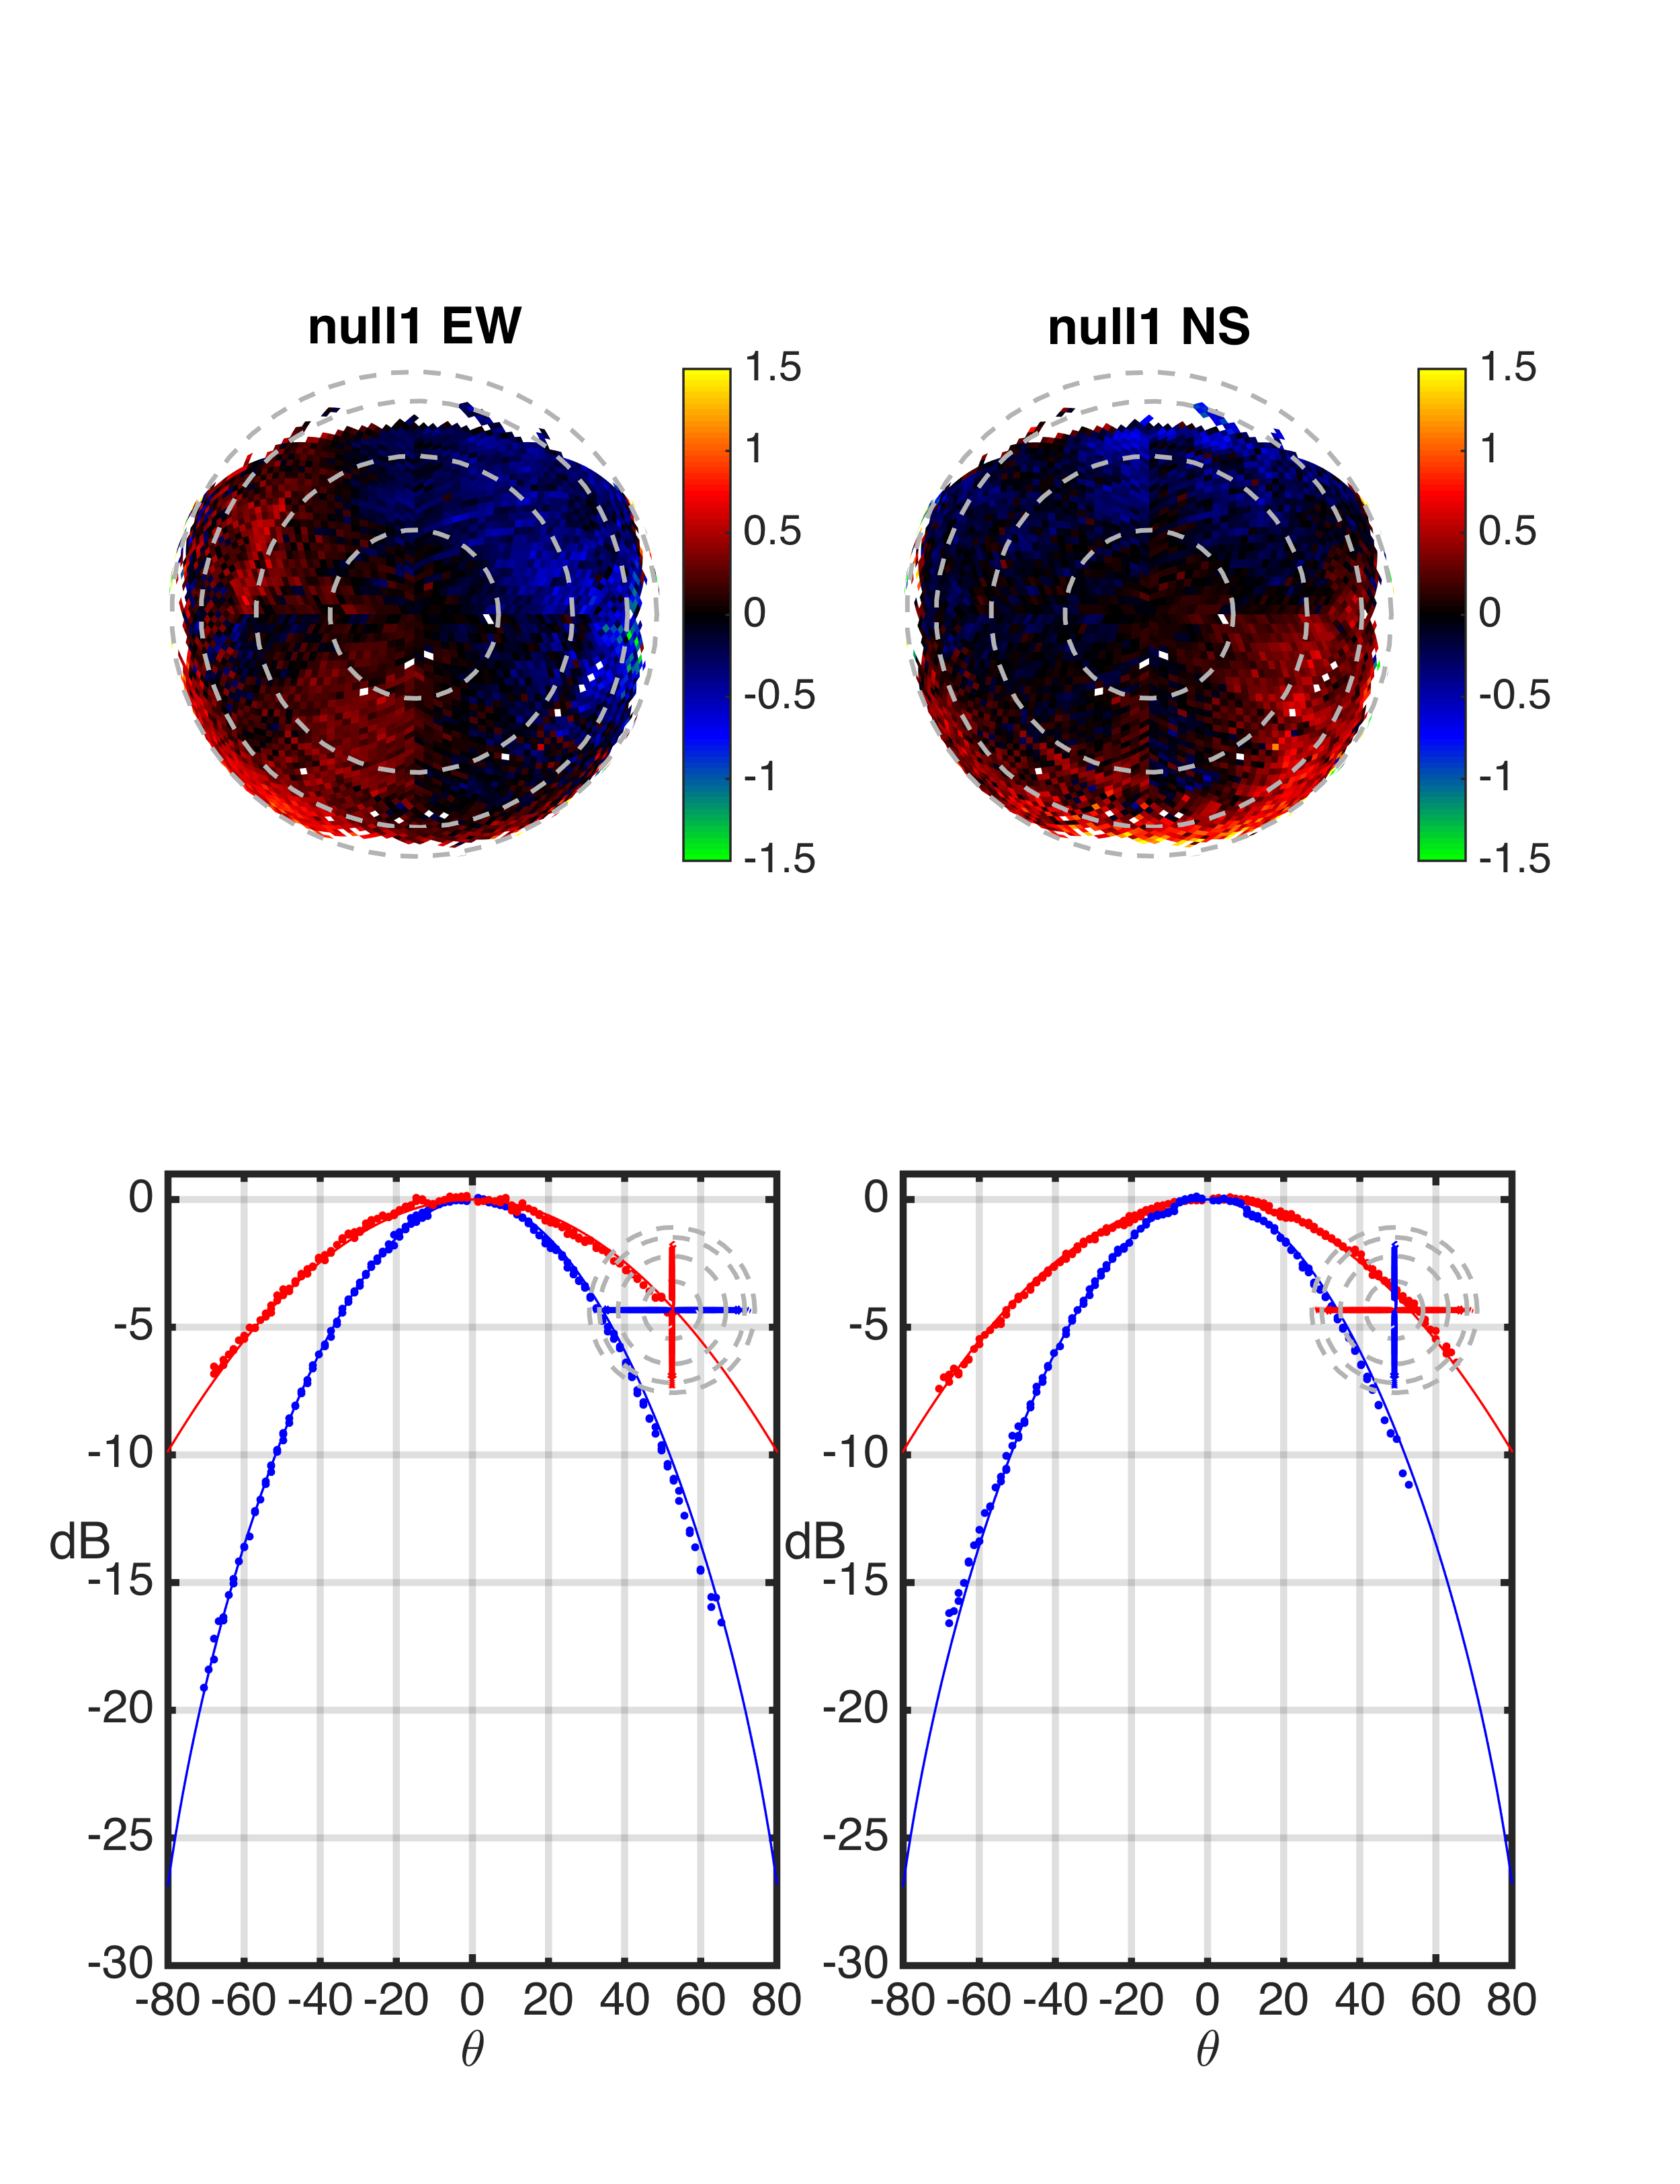
\includegraphics[width=6.5in]{null1_rel.png}
\caption{Top: ratio maps of the powers received by two reference dipoles separated by 50\,m, deployed 50\,m south of the HERA dish. Bottom: absolute beam power plots constructed by multiplying the relative power maps by a model beampattern. }
\label{fig:null1}
\end{figure*}

\begin{figure*}[h]
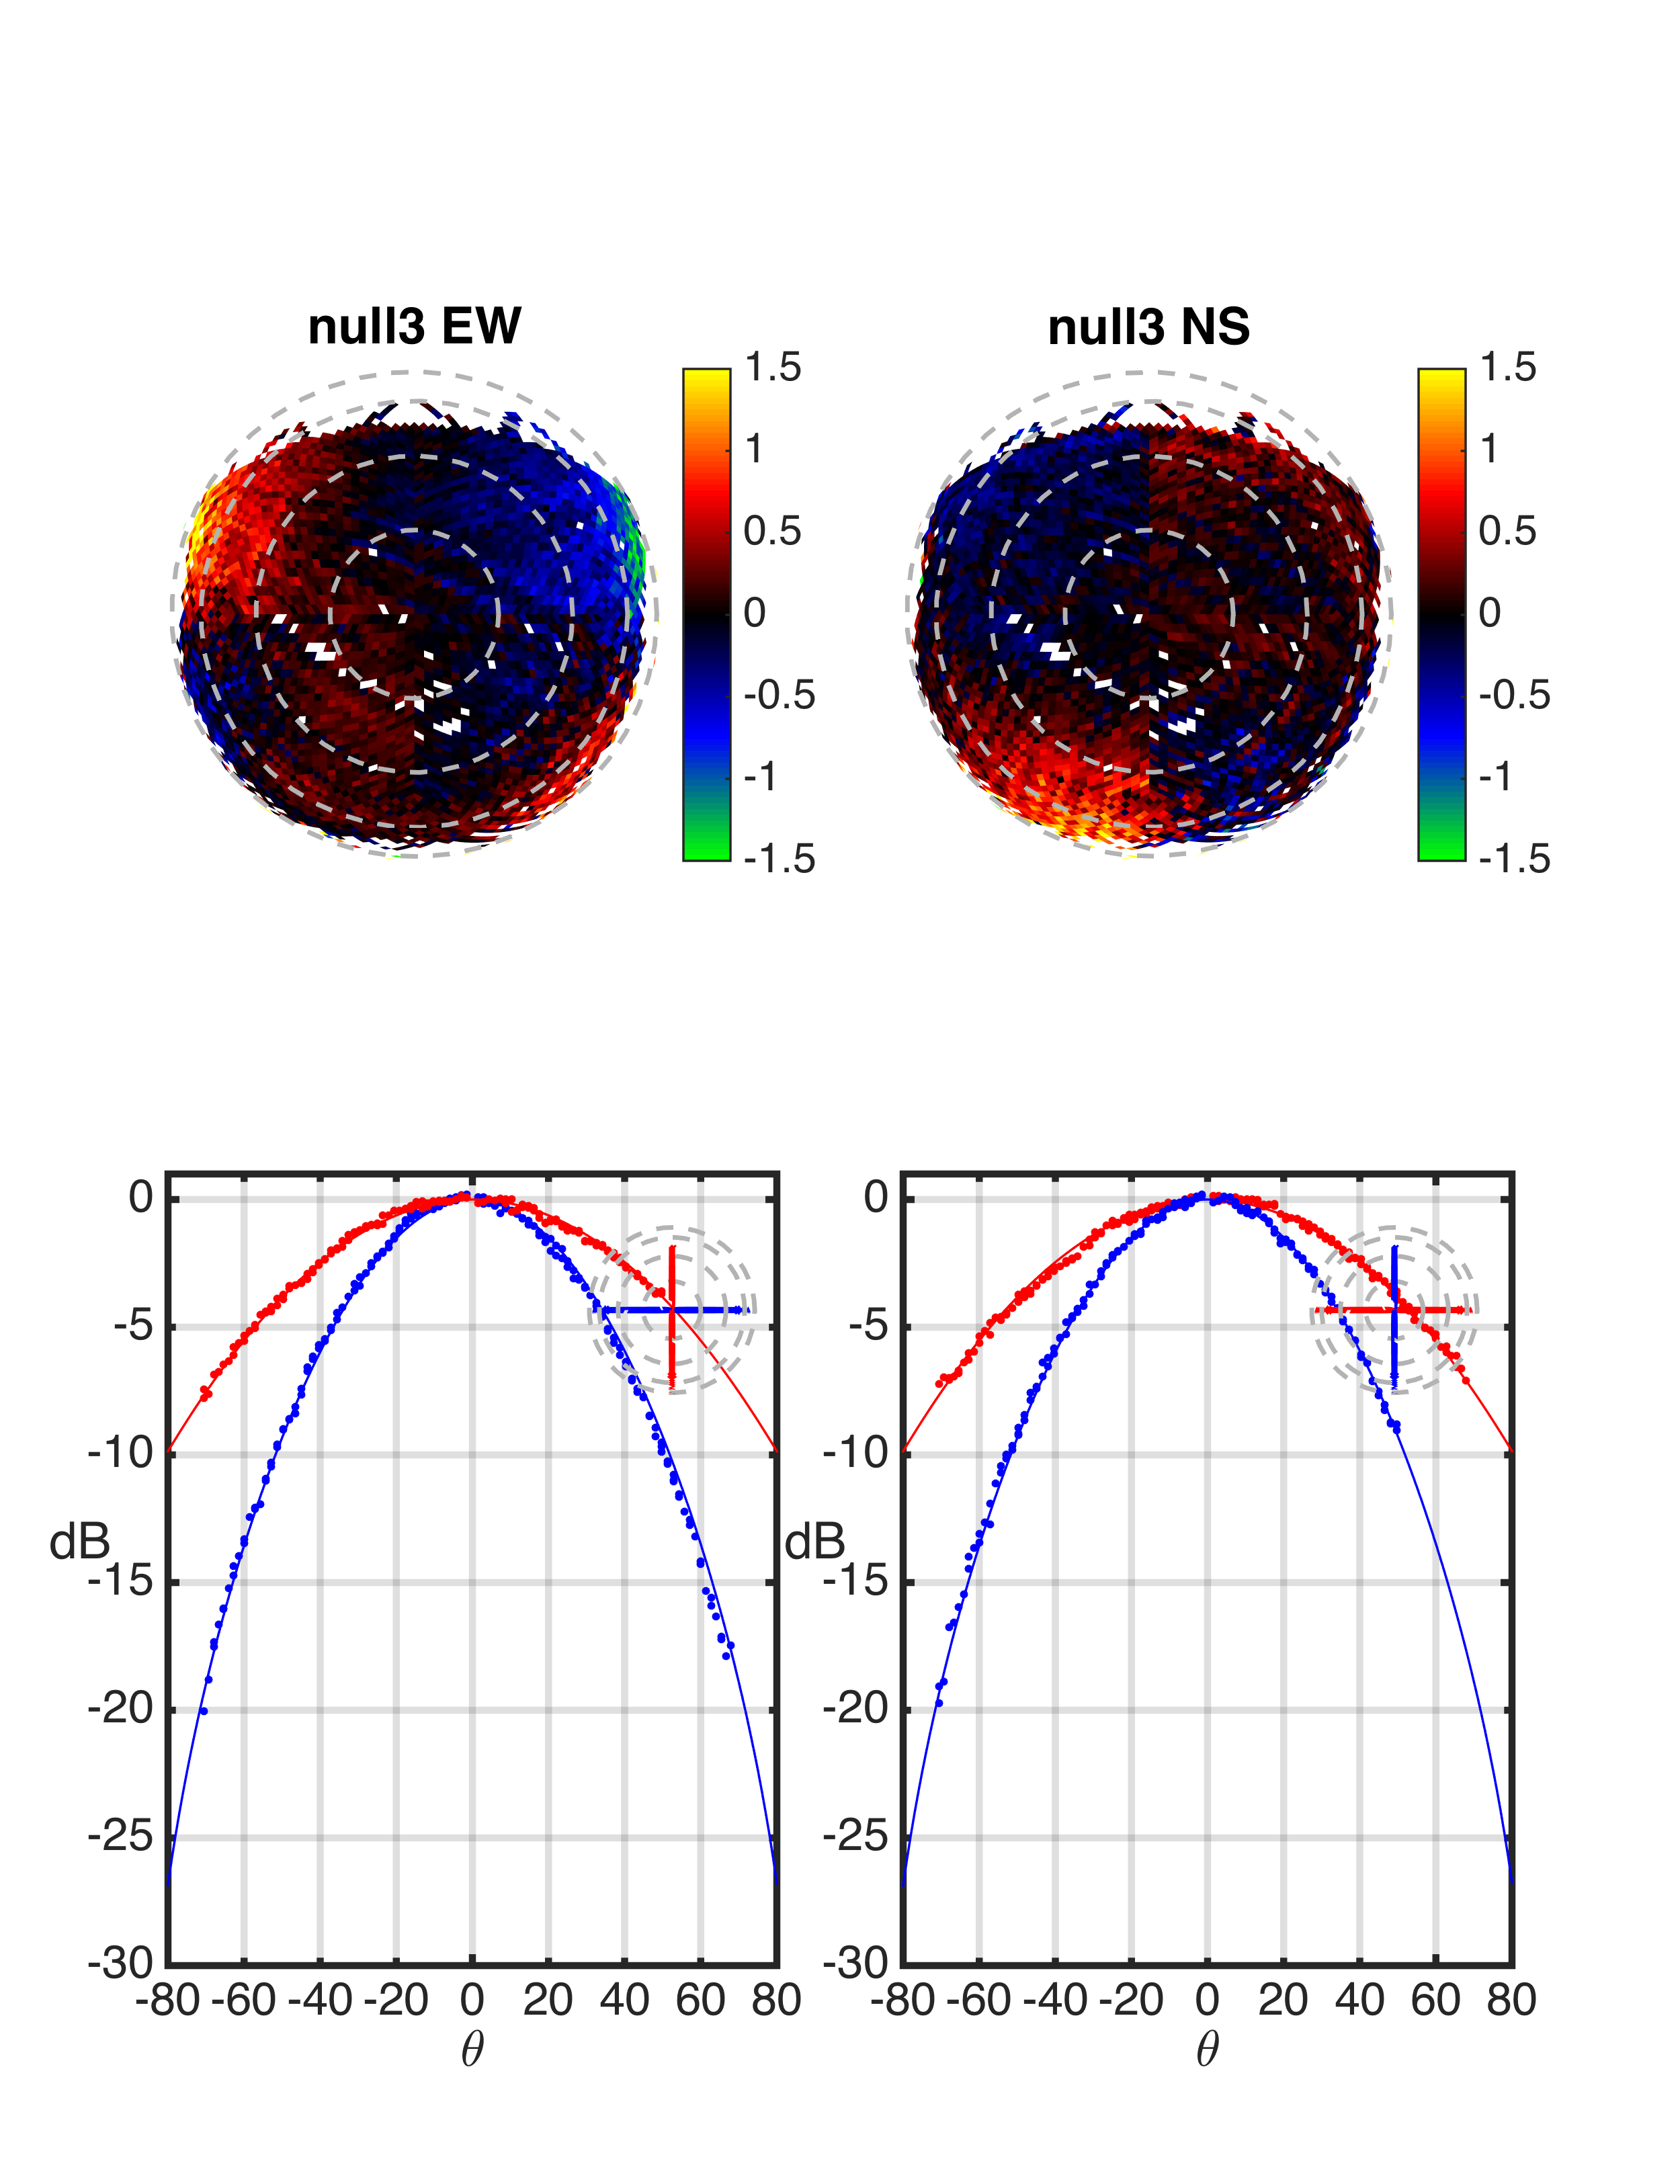
\includegraphics[width=6.5in]{null3_rel.png}
\caption{Same as the previous null experiment except the south reference dipole was moved 5\,m west. The systematics are largely unchanged.}
\label{fig:null3}
\end{figure*}

\begin{figure*}[h]
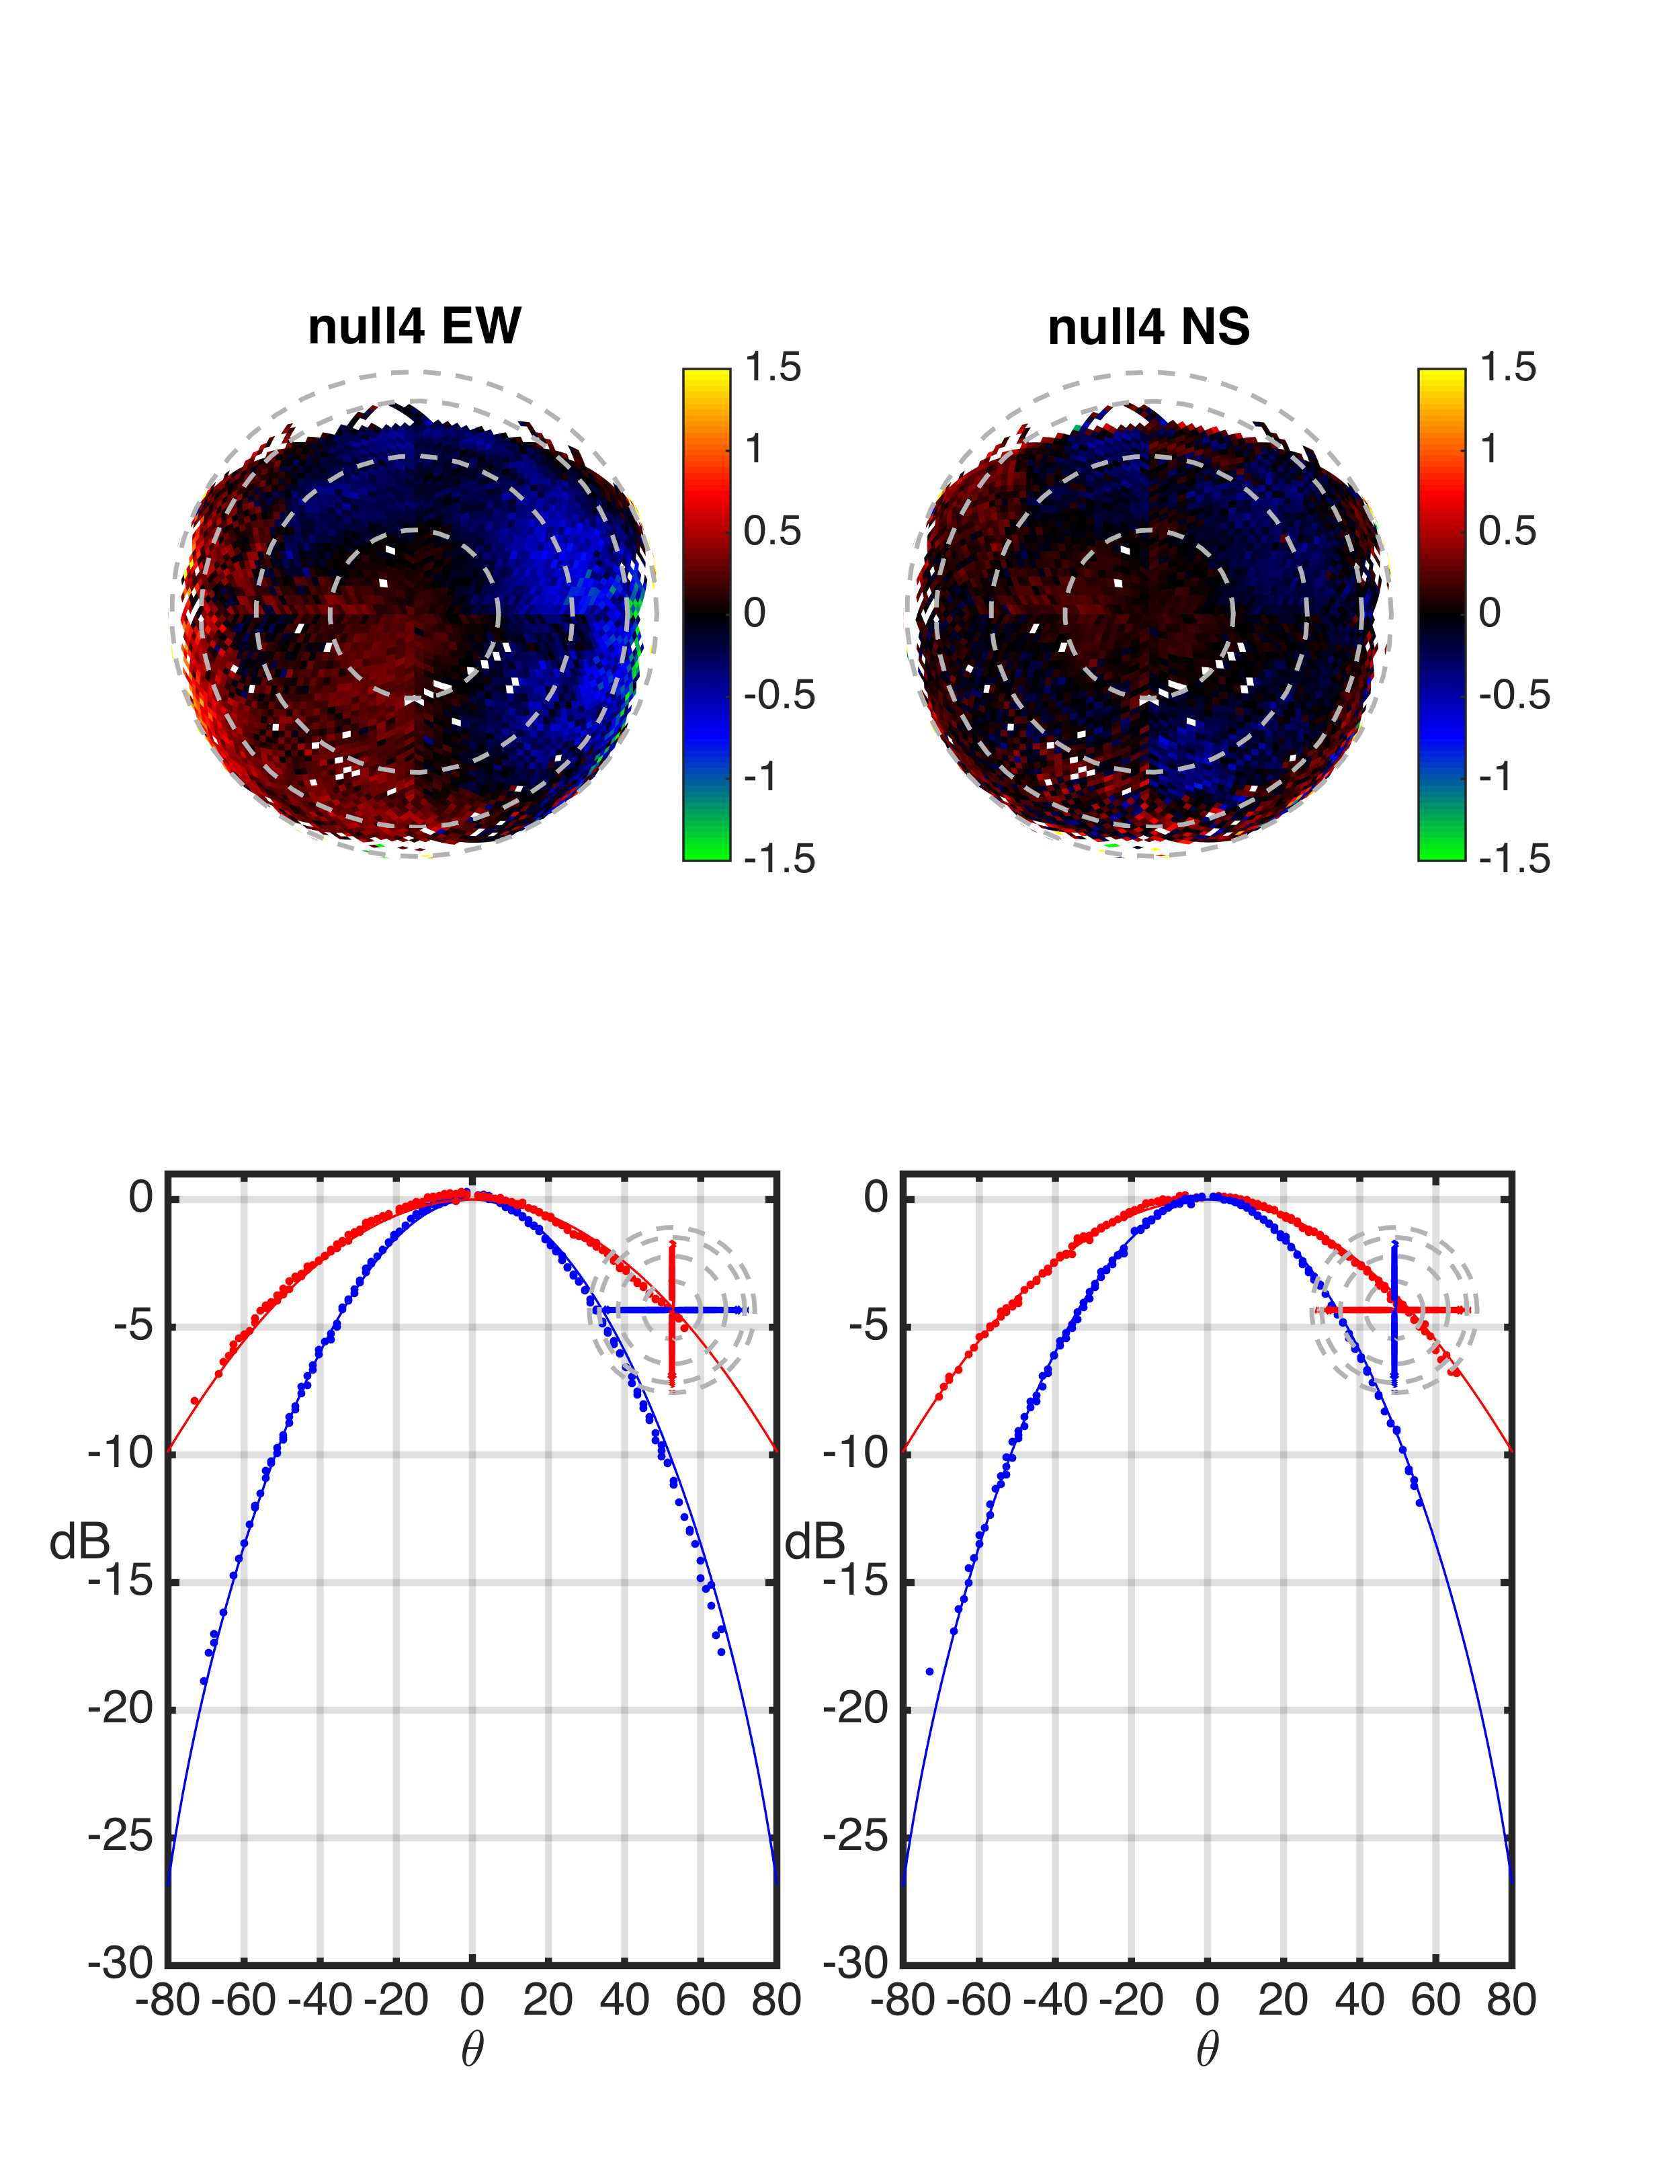
\includegraphics[width=6.5in]{null4_rel.png}
\caption{Same as the first null experiment except the reference dipoles are separated by 100\,m and deployed 100\,m south of the HERA dish. The systematics remain at the few percent level near zenith and increase to $\sim10\%$ farther out, with somewhat, but not entirely different angular structure. }
\label{fig:null4}
\end{figure*}

\section{Feed Measurements}

Accurate modeling of both the dish and feed will be essential for final dish modeling. To that end, we deploy the feed on the ground facing the sky (Figure \ref{fig:feedpic}), replacing the north-most reference antenna in the \texttt{null3} configuration, to isolate the feed power pattern. 

Figure \ref{fig:feed0} shows the measured feed beams (top panel) and slices through the E and H planes (bottom panel). Due to intermittent connection problems to the DAQ computer, we collected only 157 high signal-to-background satellite passes over a few days. Still, the data agree very well with the CST model for $\theta<55^\circ$, outside of which the E plane response starts narrows compared to the model by up to 5\,dB at $\theta=70^\circ$. Still, the data are quite sparse in these low regions due to the connection problems, and so the usual quality control cuts are likely less effective than usual. 

\begin{figure*}[h]
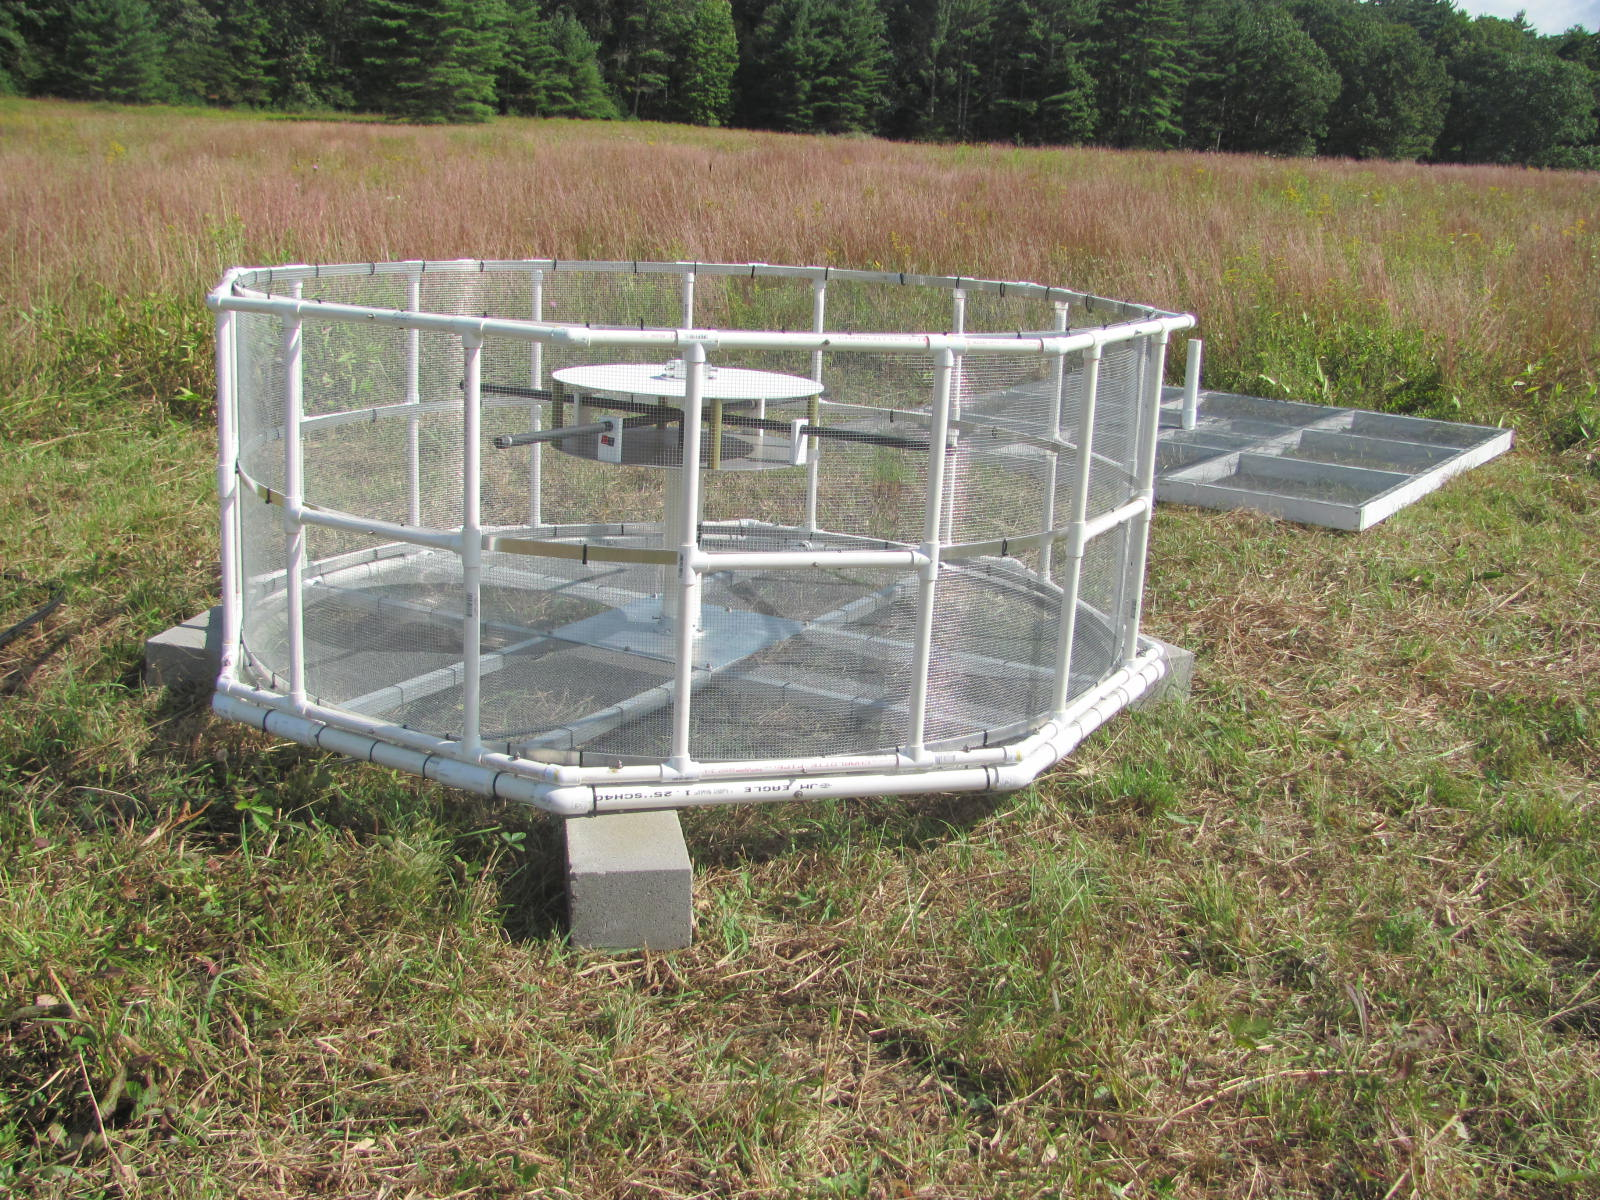
\includegraphics[width=5in]{feed.jpg}
\caption{Feed deployed on the ground, facing the sky, replacing the north-most reference antenna in the \texttt{null3} configuration. }
\label{fig:feedpic}
\end{figure*}

\begin{figure*}[h]
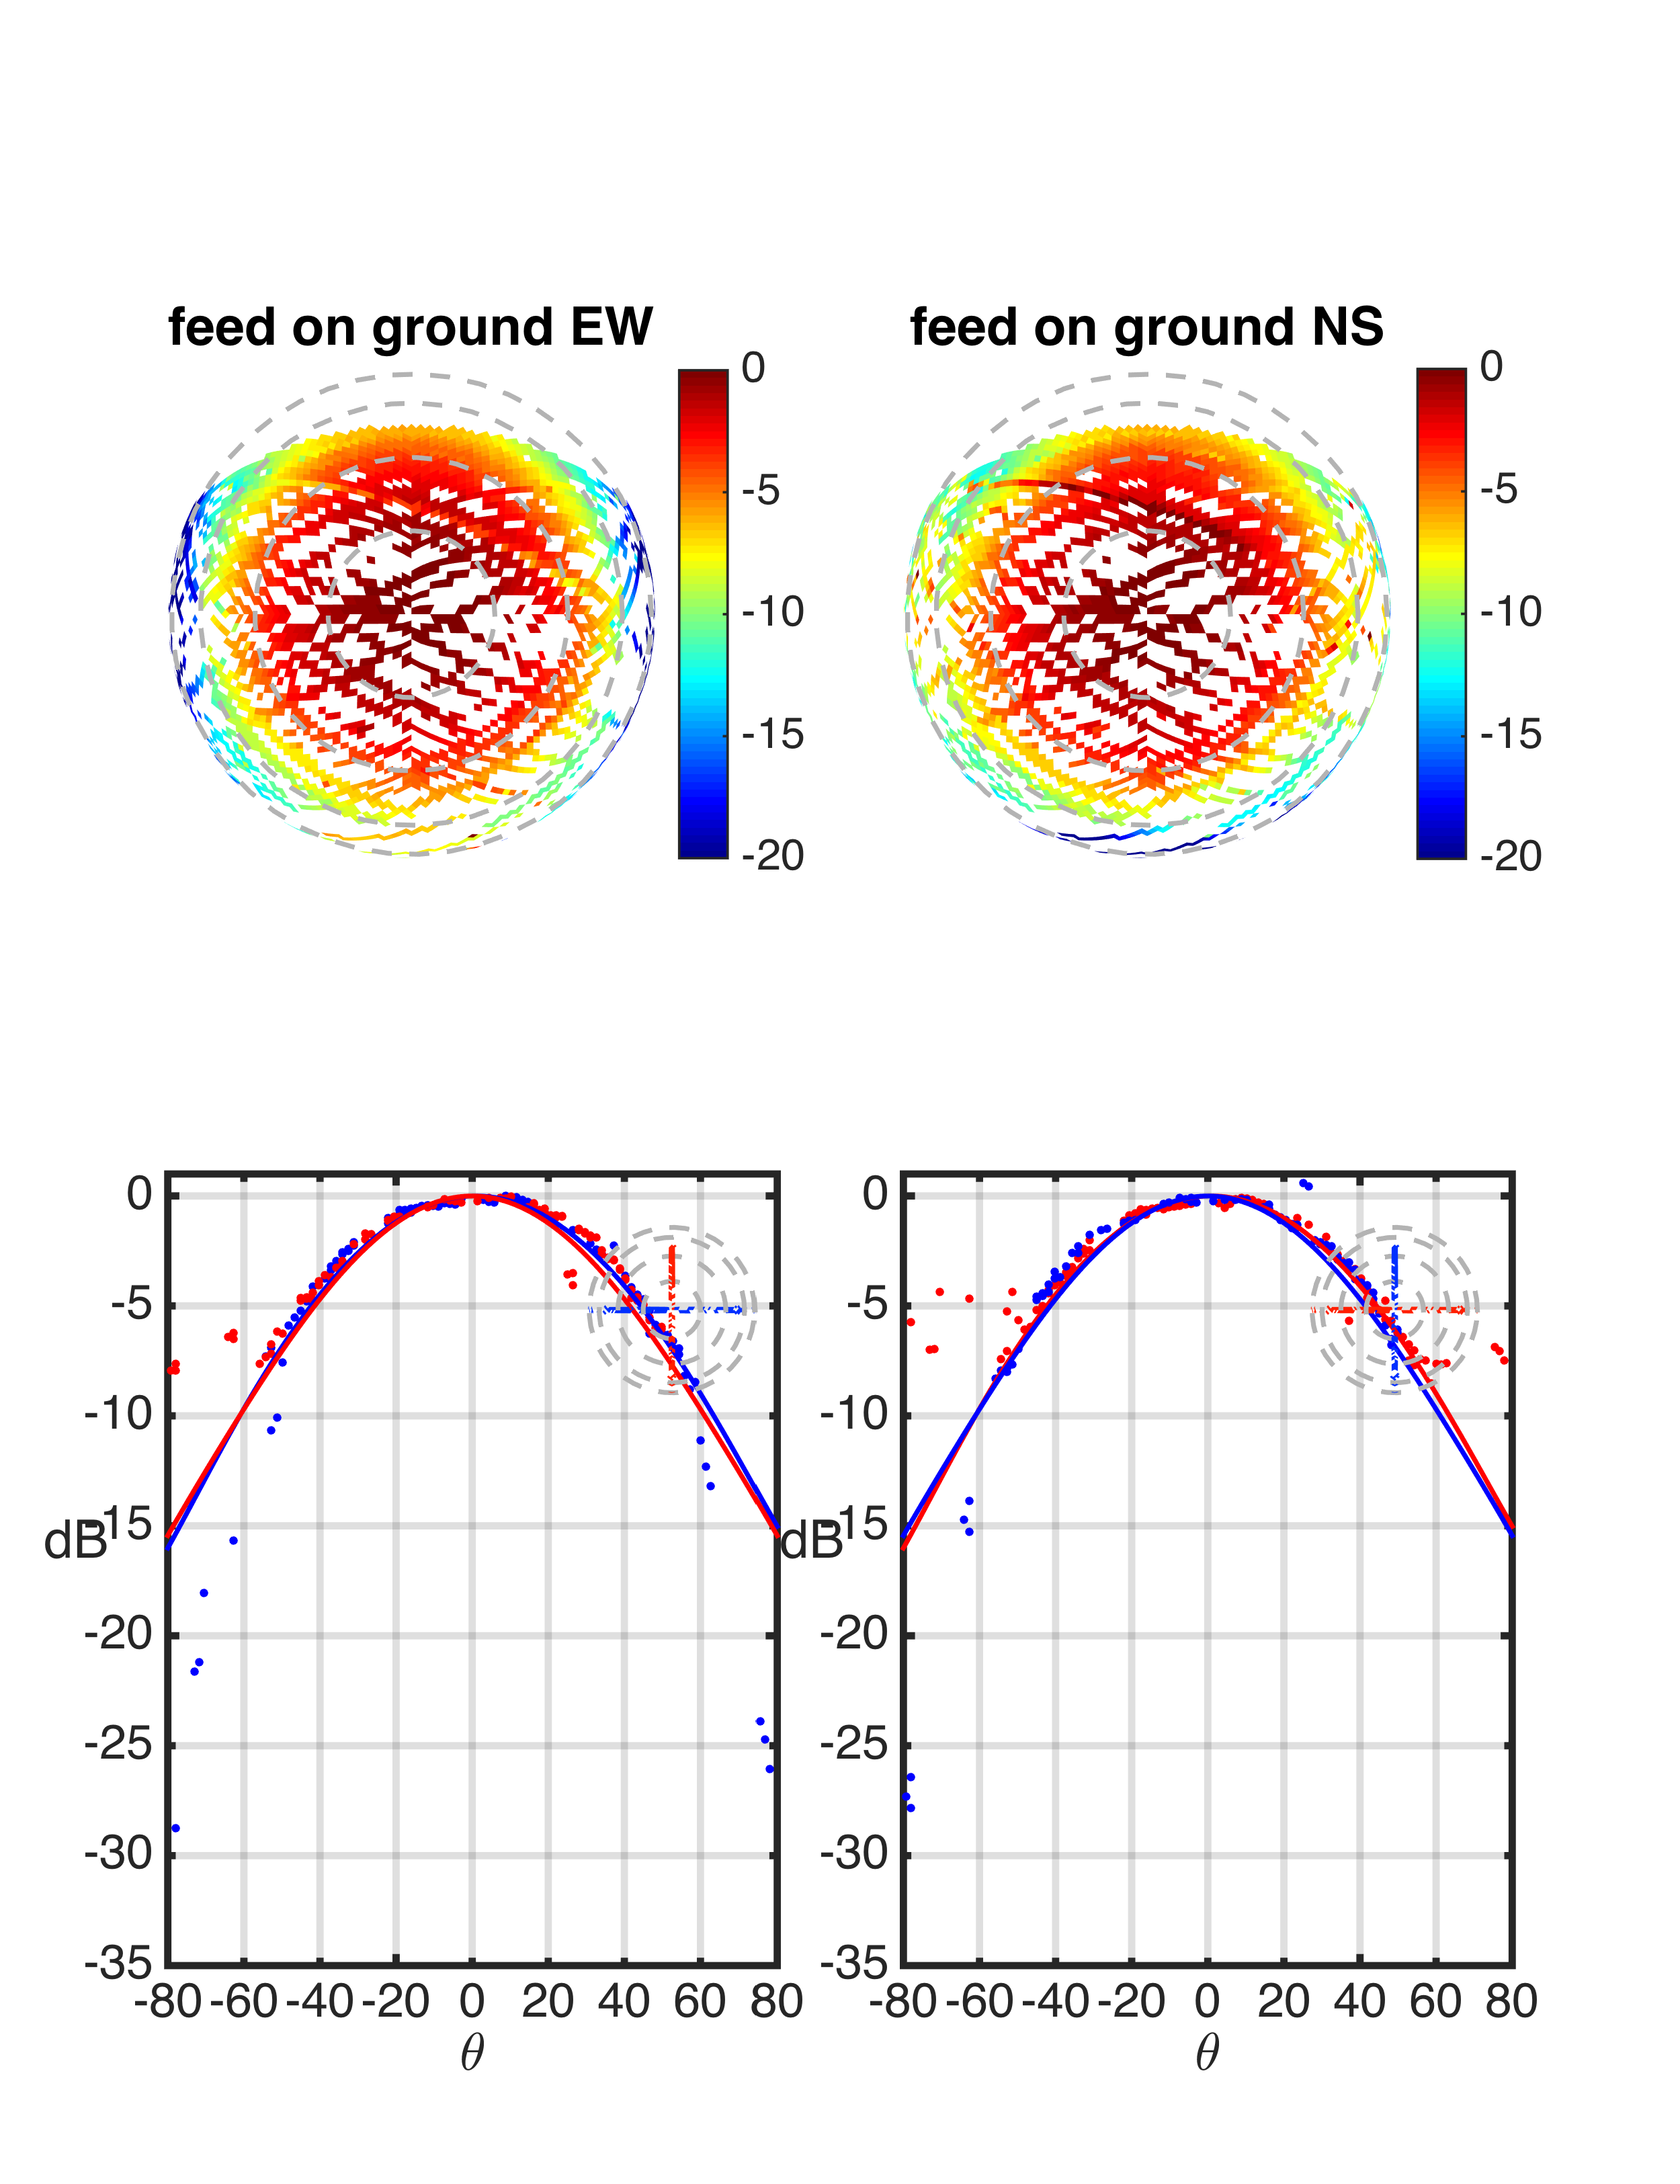
\includegraphics[width=6.5in]{feed0_abs_old_ref_model.png}
\caption{Measurements of the feed power pattern, deployed so it faces the sky. The measurements agree well with the model for $\theta<55^\circ$, but start to diverge at large zenith angles, possibly due to quality control problems due to very sparse beam sampling.}
\label{fig:feed0}
\end{figure*}

\section{Dish Characterization}

\subsection{Power pattern measurements}

Having verified the feed power pattern, we deployed feed over the dish and proceed with dish measurements. We measure the power pattern with the feed at four different heights, 4\,m, 4.5\,m, 5\,m, and 5.3\,m, chosen to probe around the nominal focus of 4.5\,m (the nominal beam) and up to the maximum height of 5.3\,m allowed by pole height and rope stresses. Heights are measured from the dish surface to the feed backplane. 

Inspecting the E and H plane slices through the measured beams (bottom panels) in Figures \ref{fig:dish3}, \ref{fig:dish1}, \ref{fig:dish2}, \ref{fig:dish4}, we generally see the main lobe narrow and the sidelobe level decrease. The improvement is also seen in the yellow and red main lobe in the beam maps (top panels) which narrow and approach the expected orientations: the EW (NS) main lobe is elongated in the NS (EW) direction. The last lift produced the smallest change in the beam suggesting it is quite near the best focus. 

The sky coverage in these dish measurements extends out to typically $\theta\sim50-60^\circ$. Beyond that the ORBCOMM flux is sufficiently attenuated relative to diffuse galactic emission that a power ratio measurement between the two antennas is no longer a clean probe of their gains in the direction of the satellite. At these zenith angles, the beam sidelobes are roughly -30\,dB, and seem to be trending downward at the edge of the measured region.

\begin{figure*}[h]
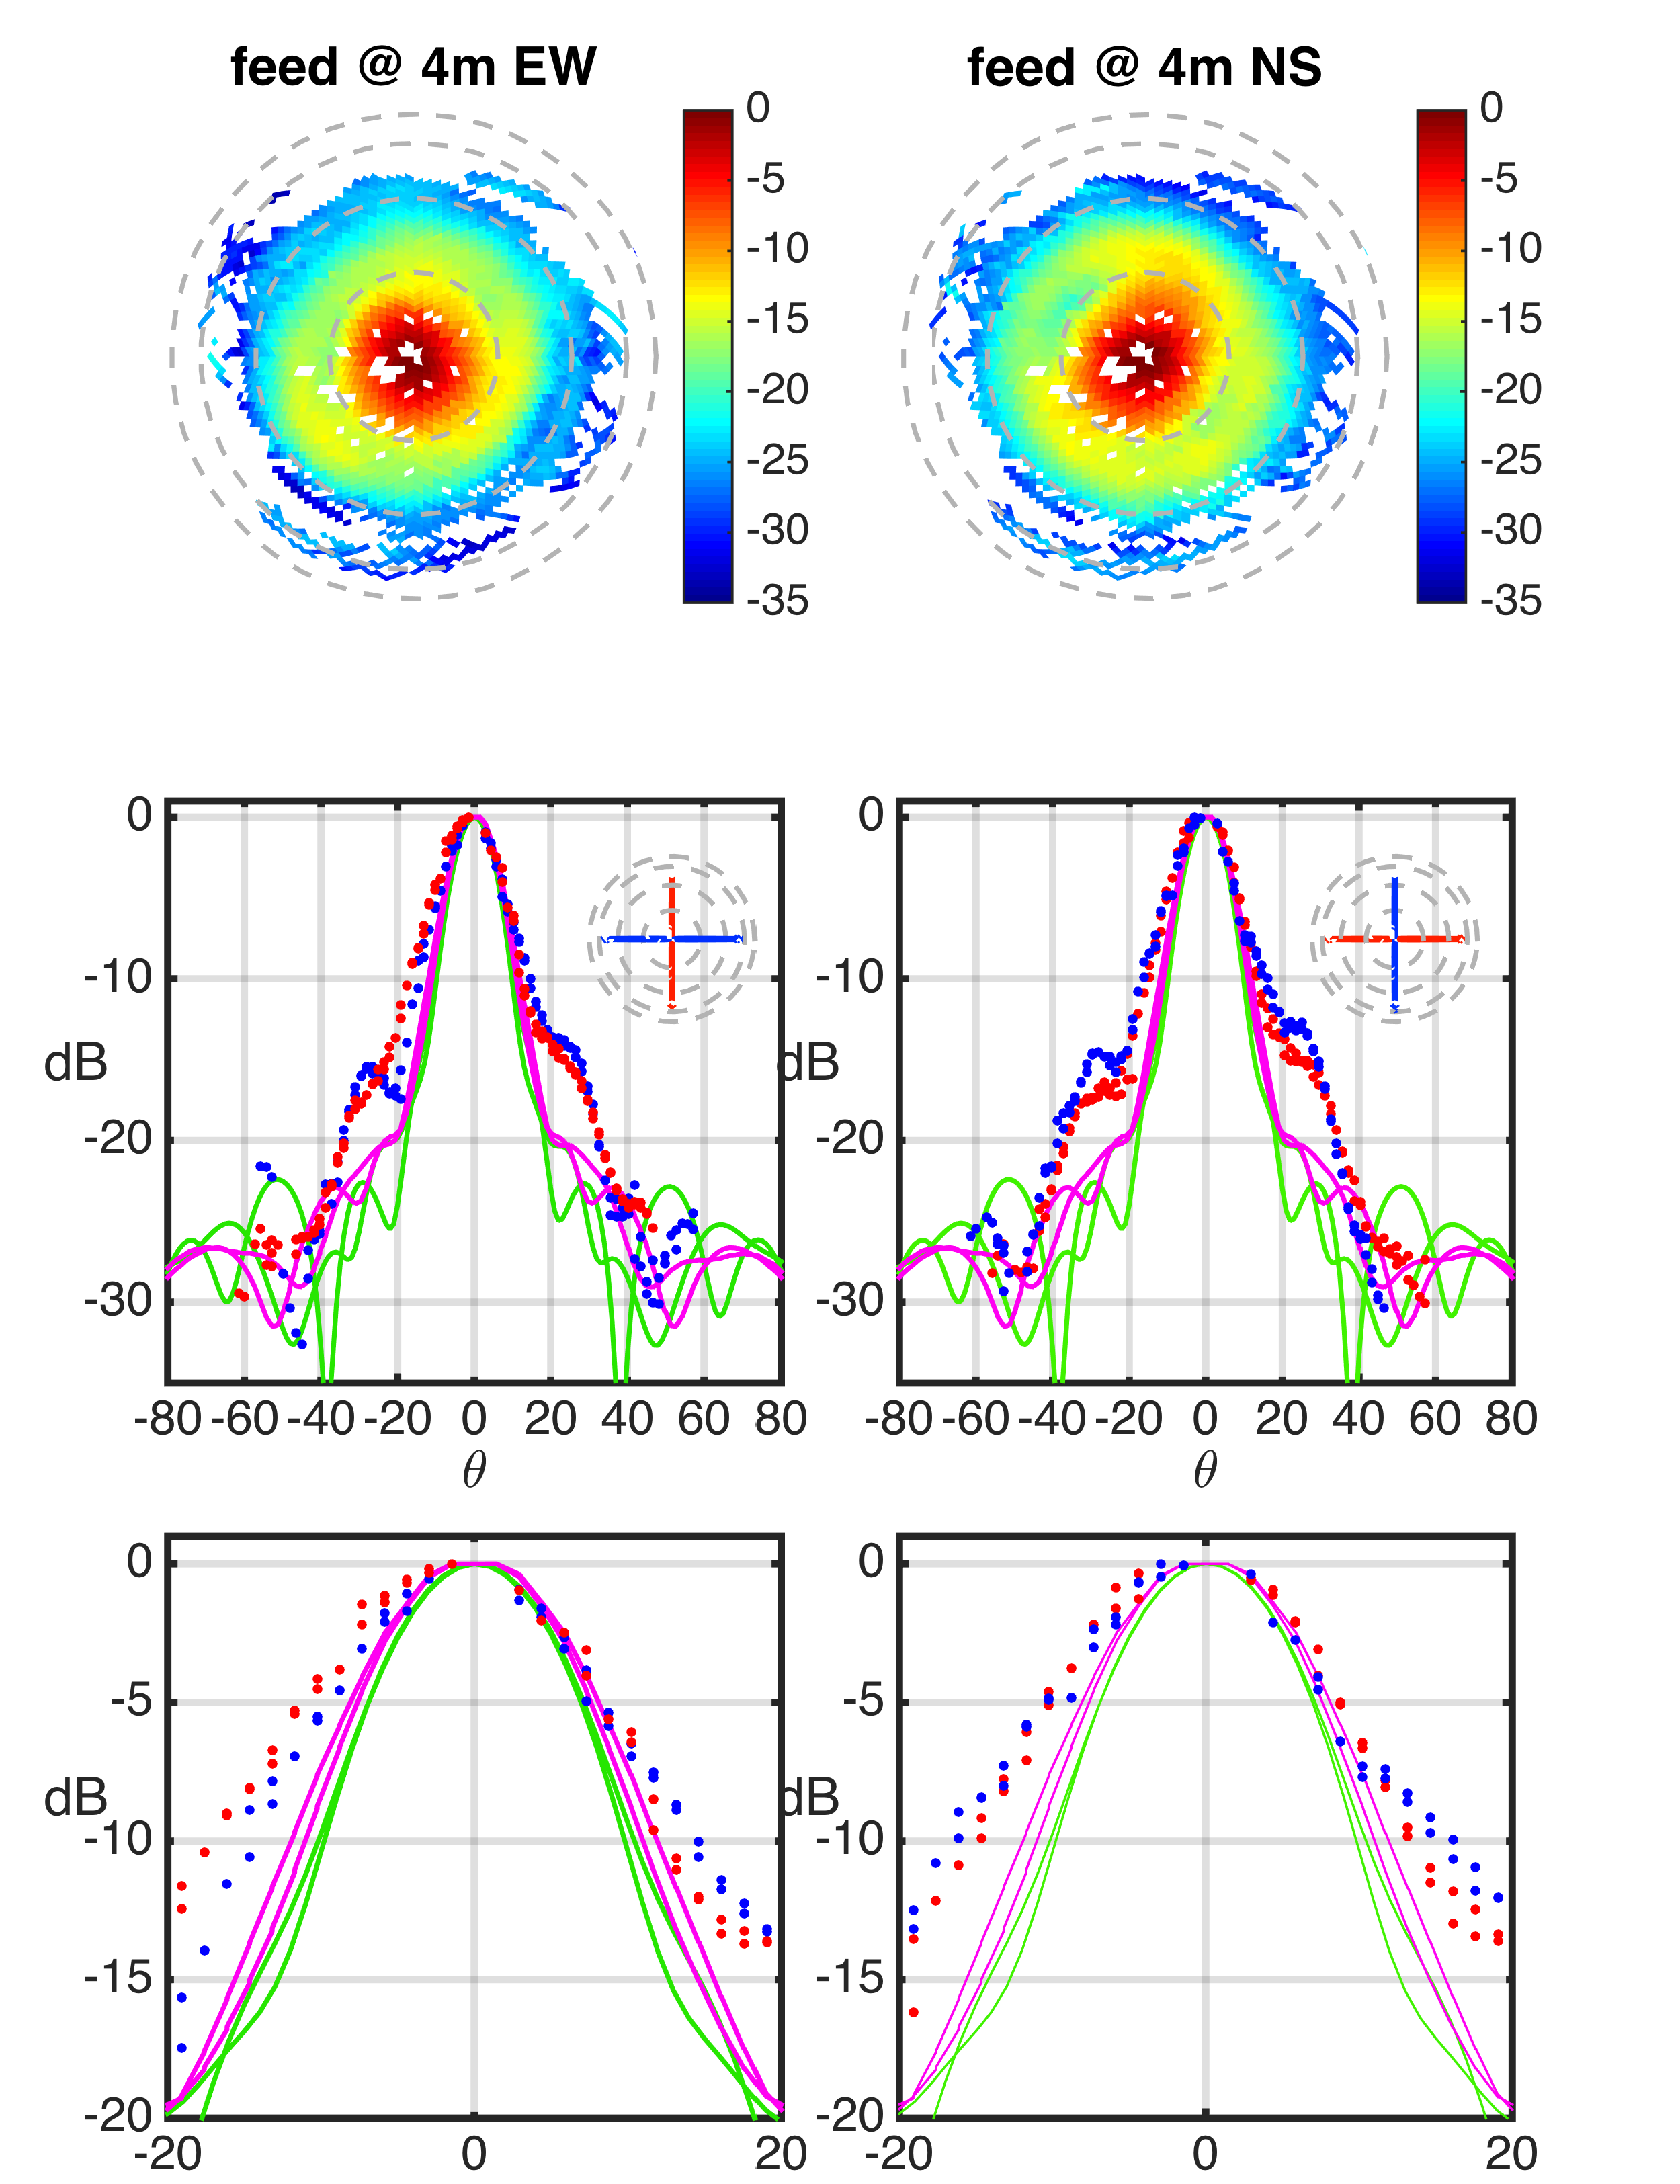
\includegraphics[width=6.5in]{dish3_abs_old_ref_model.png}
\caption{Dish power pattern with the feed lowered 0.5\,m below nominal focus.}
\label{fig:dish3}
\end{figure*}

\begin{figure*}[h]
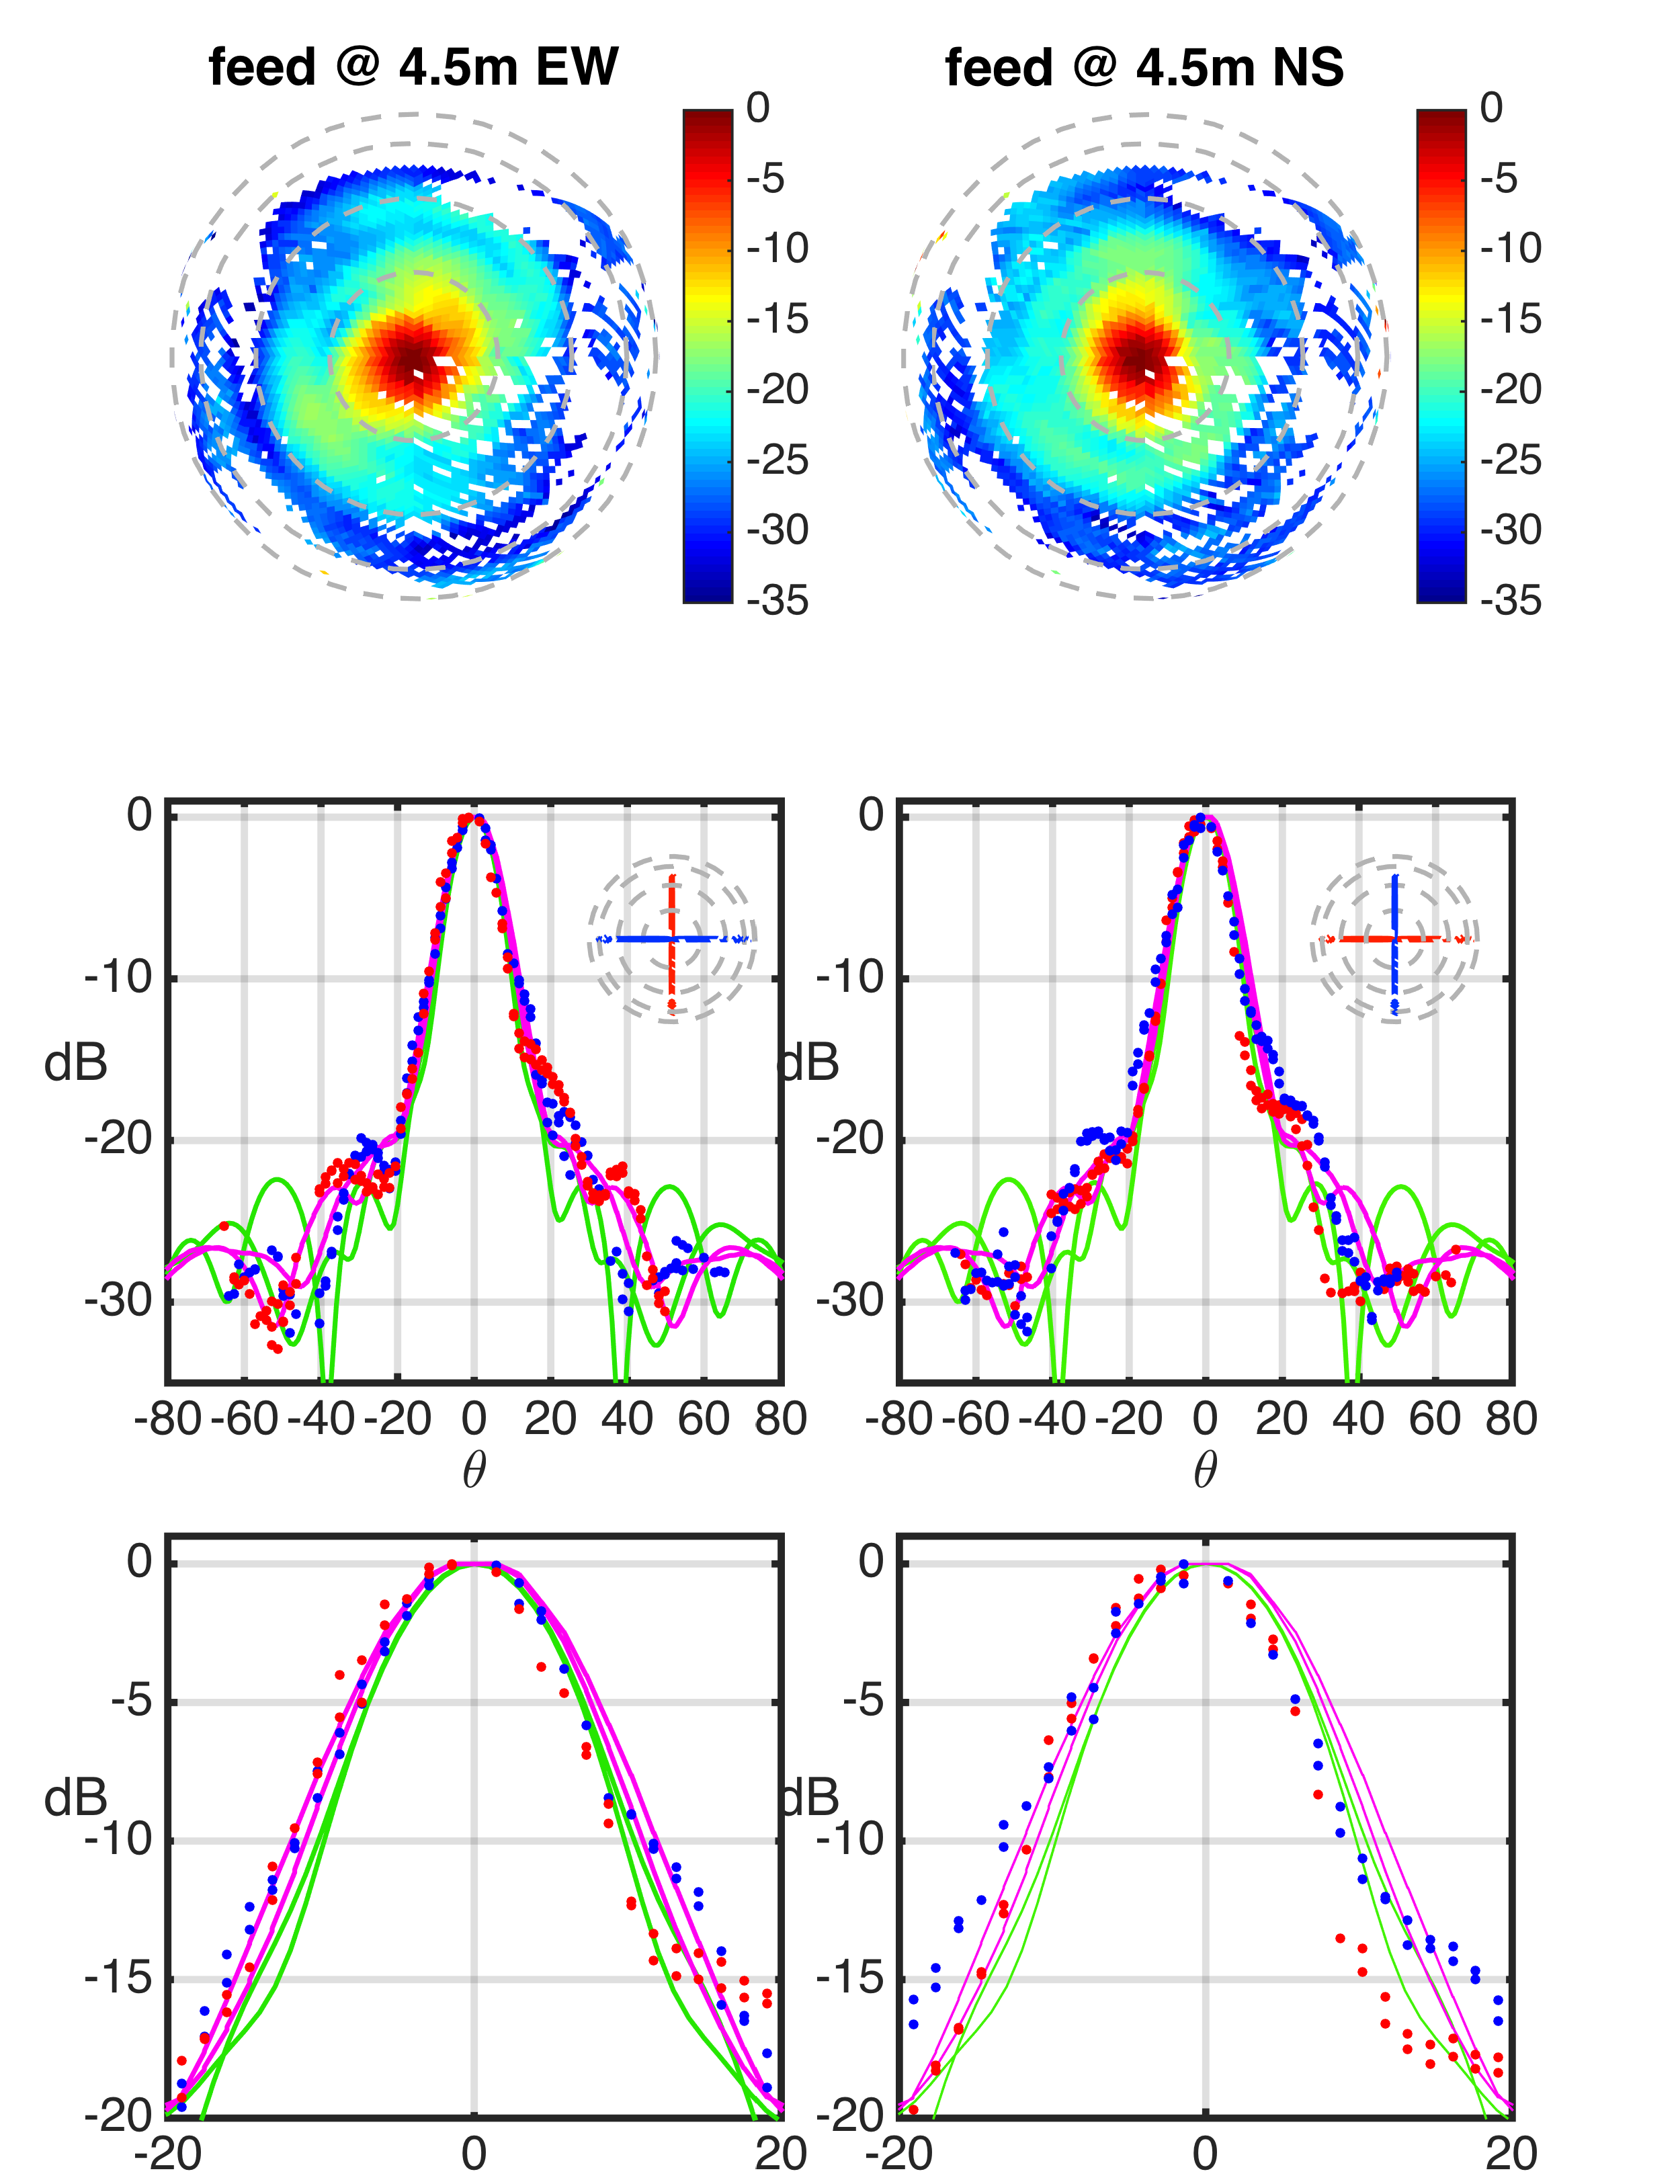
\includegraphics[width=6.5in]{dish1_abs_old_ref_model.png}
\caption{Dish power pattern with the feed at the nominal focus of 4.5\,m.}
\label{fig:dish1}
\end{figure*}

\begin{figure*}[h]
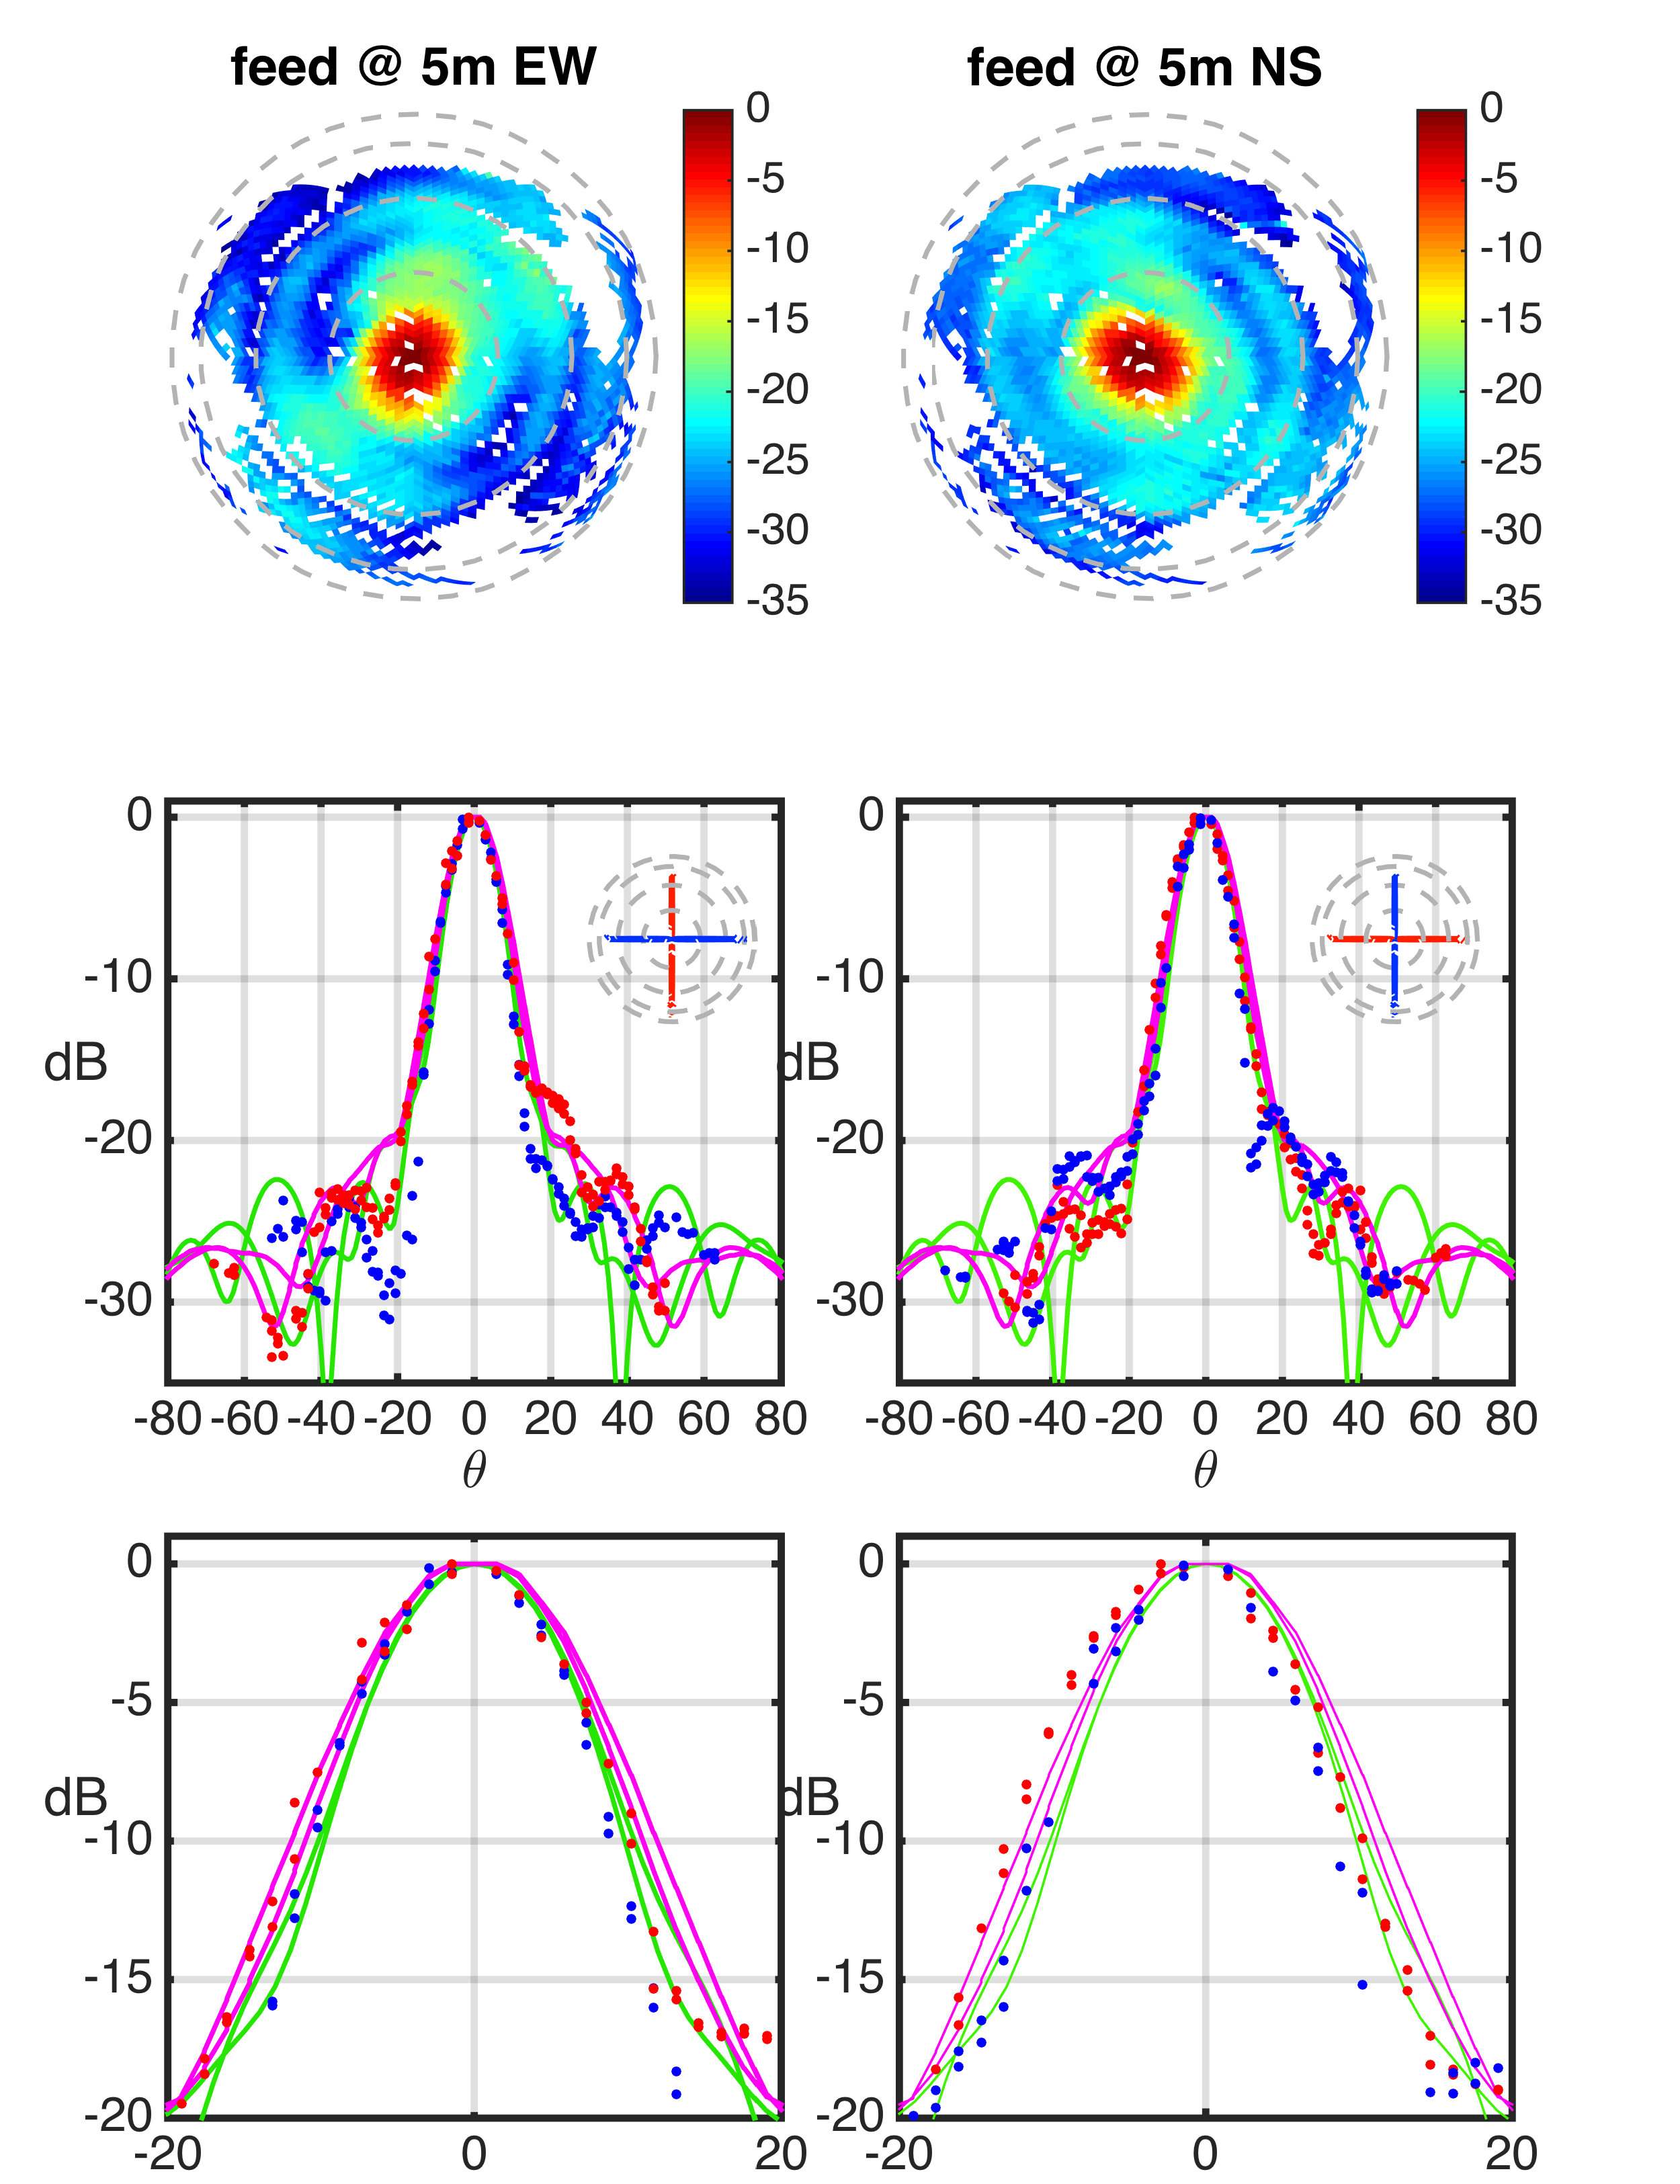
\includegraphics[width=6.5in]{dish2_abs_old_ref_model.png}
\caption{Dish power pattern with the feed raised 0.5\,m above nominal focus.}
\label{fig:dish2}
\end{figure*}

\begin{figure*}[h]
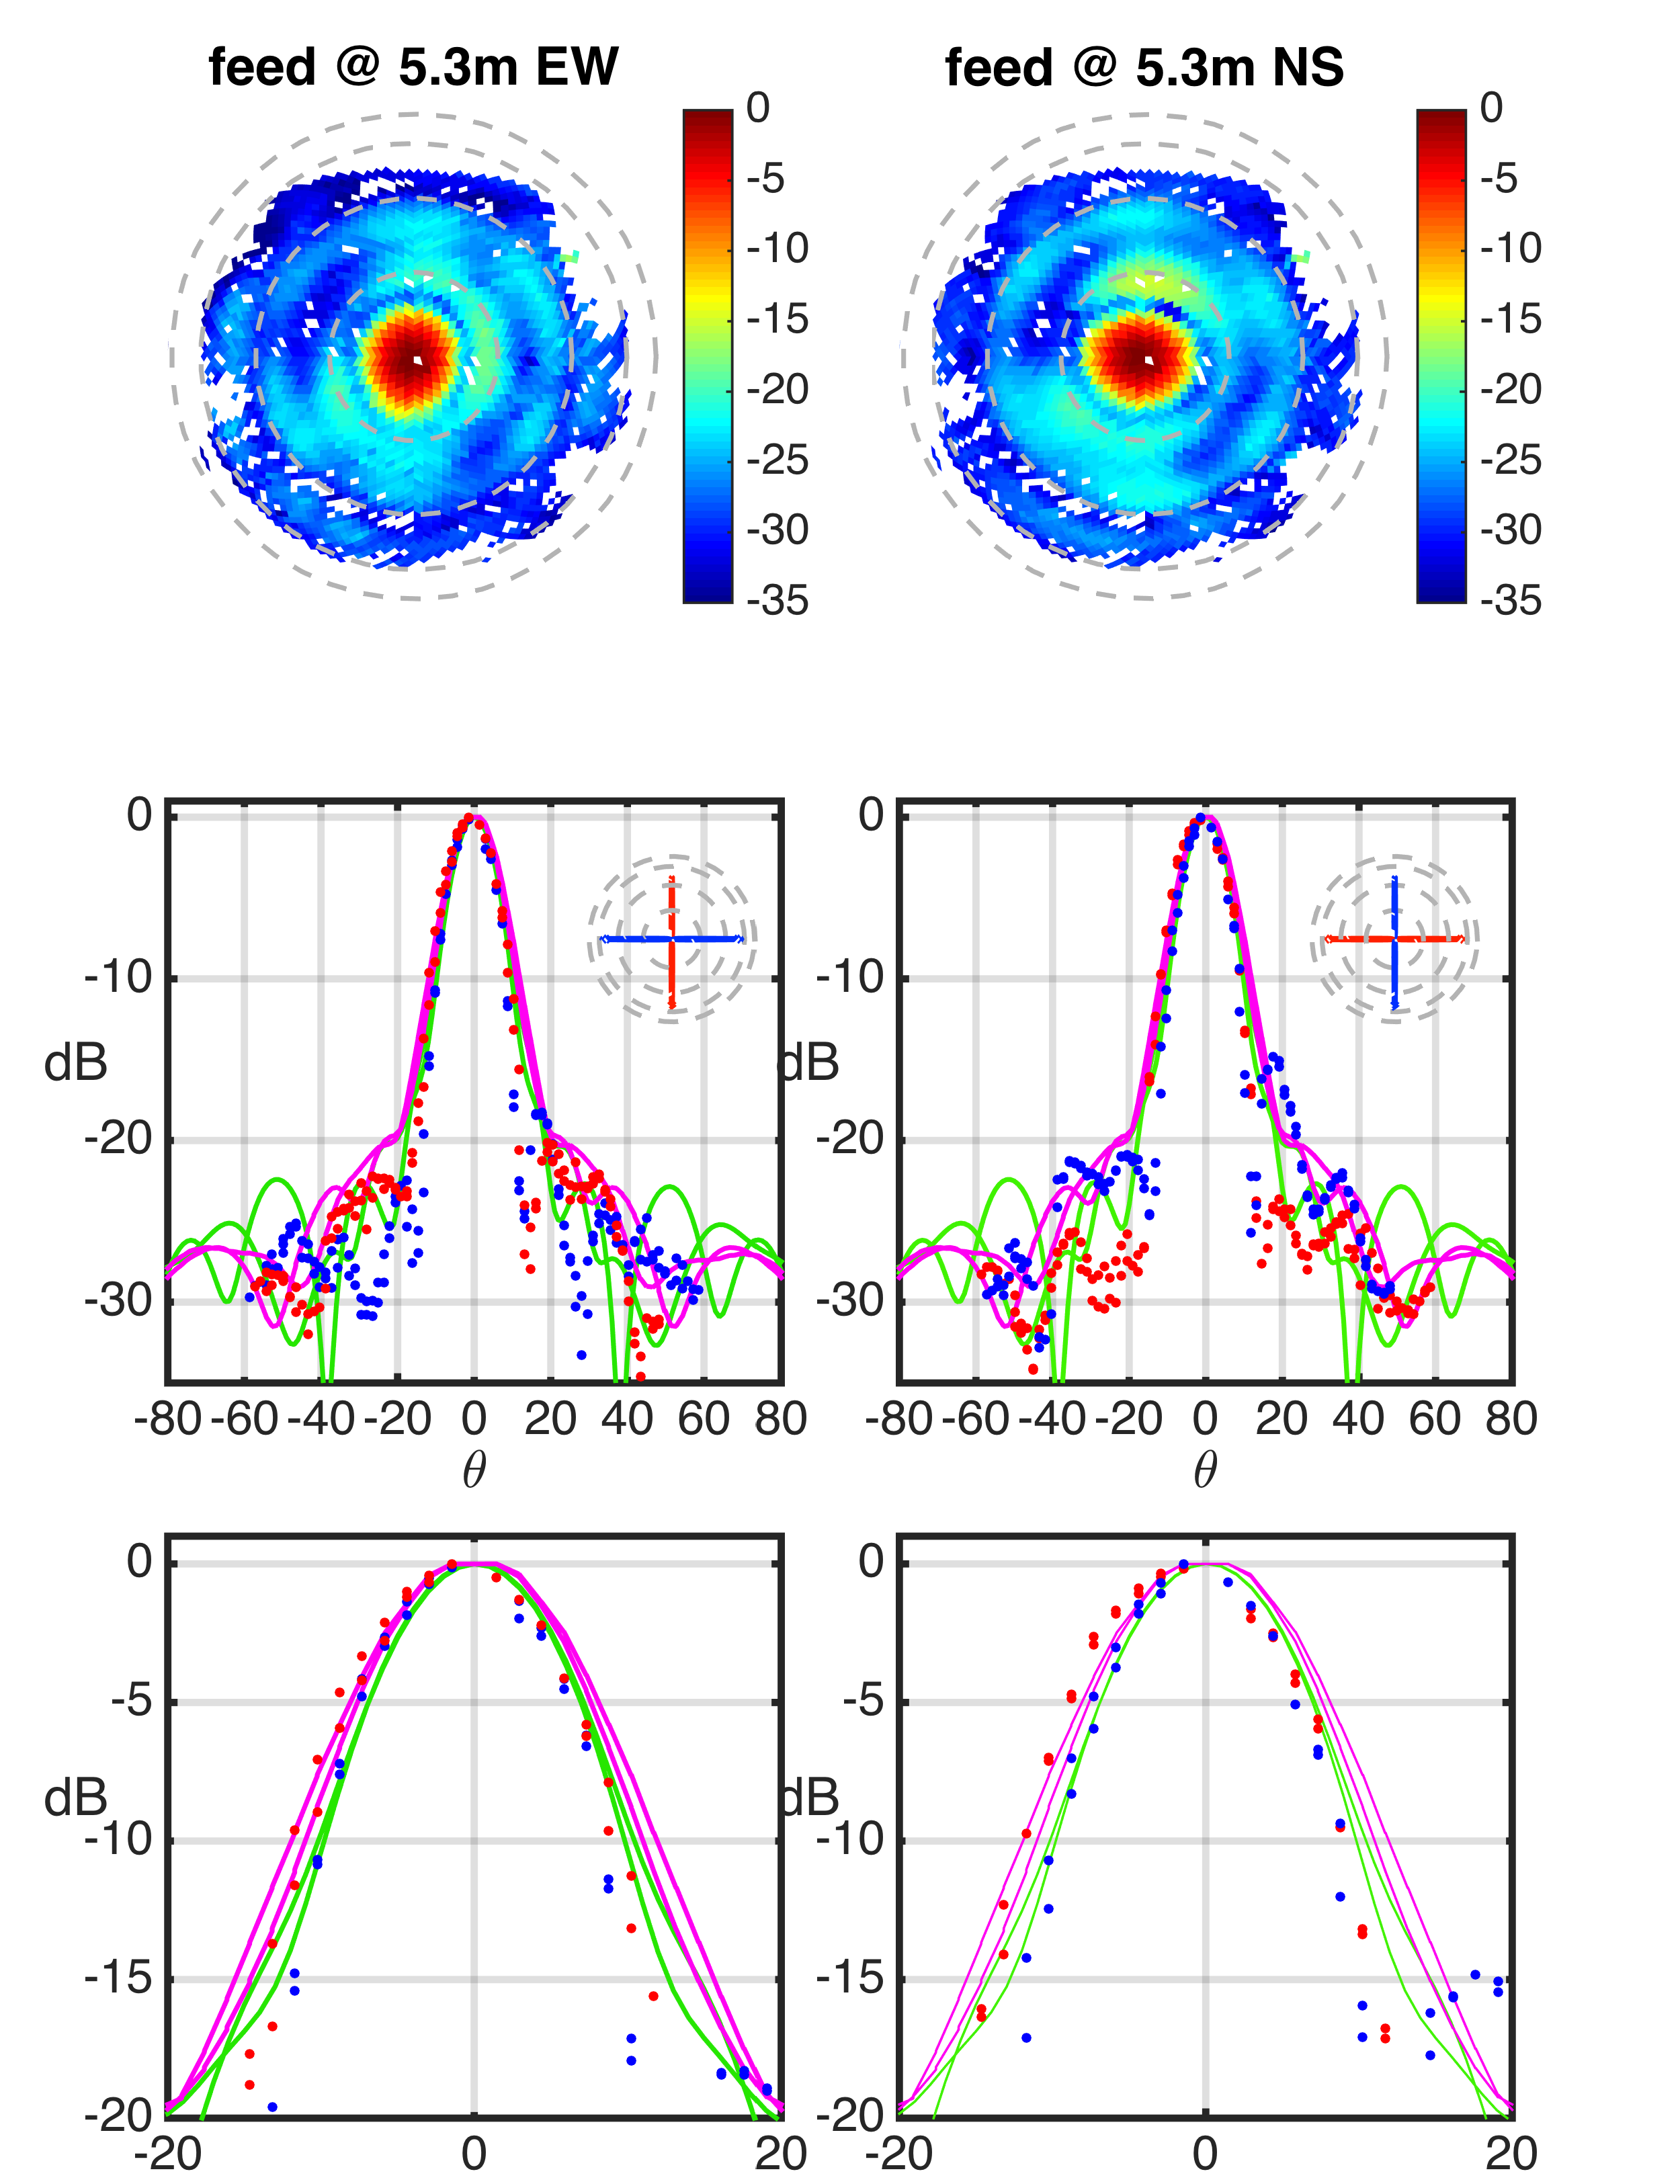
\includegraphics[width=6.5in]{dish4_abs_old_ref_model.png}
\caption{Dish power pattern with the feed raised to its maximum height of 0.8\,m above nominal focus.}
\label{fig:dish4}
\end{figure*}

In order to compute beam collecting areas and assess foreground leakage we require a beam covering the entire visible sky. For each measured dish beam, we interpolate over the unmeasured cells at $\theta\lesssim60$, then extrapolate outward to the horizon. This amounts to a smooth continuation of the beam response at the same $\sim-30$\,dB level suggested by the fringes of our measurements. We take this as a first possible model of the full sky dish beam, and construct a second with a gaussian cutoff at $\theta=60^\circ$ with $\sigma=2.5^\circ$, the pair of which span the space of likely horizon responses. This procedure is depicted in Figure \ref{fig:interpbeams} where we plot the measured nominal focus beam, the beam after interpolation and extrapolation, and the beam after applying the gaussian cutoff. Figure \ref{fig:interpbeamsslice} shows the interpolated/extrapolated beam and the beam with the cutoff along with various models to illustrate the different horizon responses more clearly.

\begin{figure}[h]
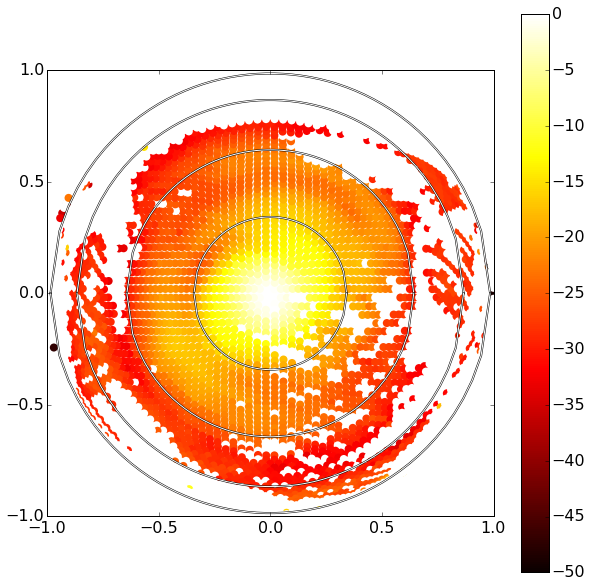
\includegraphics[width=3.5in]{measbeam_raw.png}
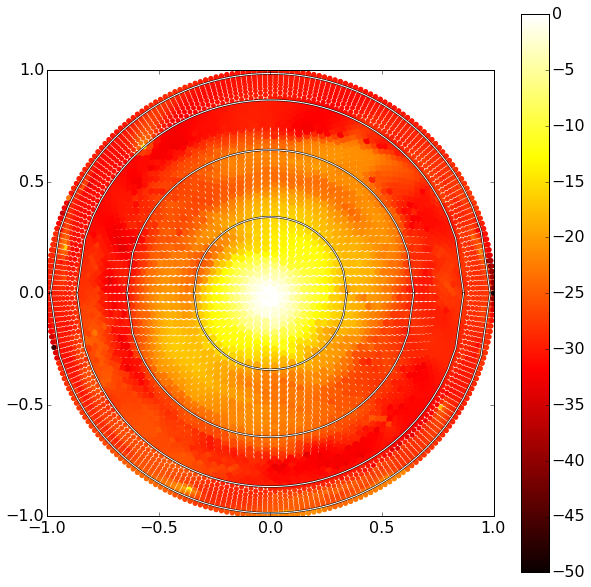
\includegraphics[width=3.5in]{measbeam_interp.png}
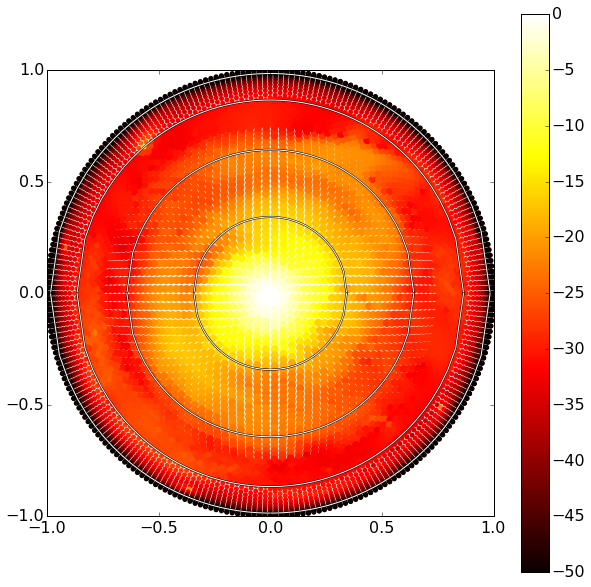
\includegraphics[width=3.5in]{measbeam_interp_expcutoff.png}
\caption{We construct full sky beams as required for Section \ref{sec:sci} by starting from the nominal focus beam (top left), interpolating over unobserved cells at $\theta\lesssim60^\circ$ and extrapolating to the horizon (top right), and applying a gaussian cutoff starting at $\theta=60^\circ$ with $\sigma=2.5^\circ$ (bottom left). These last two beams span the space of likely horizon responses.}
\label{fig:interpbeams}
\end{figure}

\begin{figure}[h]
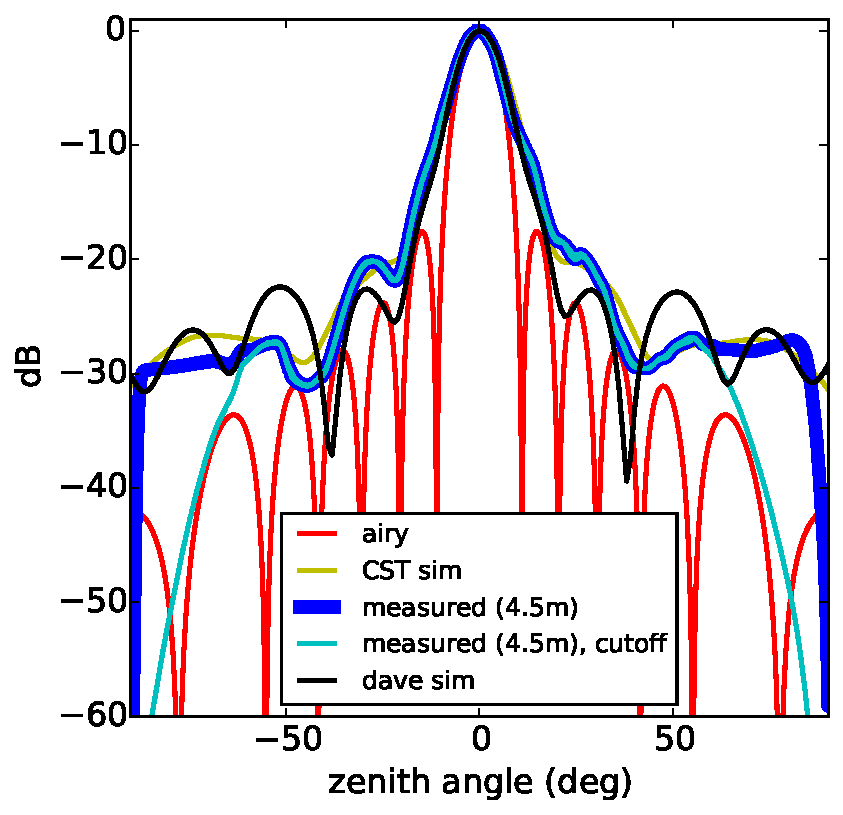
\includegraphics[width=3.5in]{ew_beams_slice.pdf}
\caption{We plot the interpolated/extrapolated measured nominal focus  beam itself (blue), and with the gaussian cutoff (cyan), along with various model beams to illustrate the varying horizon responses. }
\label{fig:interpbeamsslice}
\end{figure}

To illustrate the results of these smoothing operations we plot slices through the nominal focus dish beam along with the three model beams discussed in Sec. \ref{sec:dishmodels}. The H (E) plane slice of the main lobe is shown at the top (bottom). The plots in the left side zoom in on the main lobe, while those on the right show a zoomed out view of the entire sky pattern. 

\subsection{Collecting Area}

The collecting area of the antenna is related to the power pattern by the ratio of the beam gain to its beam-weighted solid angle as
\begin{equation}
	A=\frac{\lambda^2 B(0,0)}{\int B(\theta,\phi)d\Omega}
\end{equation}
We evaluate the collecting area for four of the beams discussed above and present the numbers in Table 1. We are unable to quantify the collecting area of the beam from Dave's simulation because it was run at too coarse an angular resolution. For the measured beams, we compute the collecting area using the interpolated/extrapolated beams with and without the gaussian cutoff at $\theta=60^\circ$.

 \begin{table}[h]
 \caption{ \label{table:collectingareatable}Collecting area (m$^2$) for modeled and measured dish beams at 137\,MHz. For measured beams, we calculate the collecting area after interpolation/extrapolation, also with the $60^\circ$ gaussian cutoff (in parentheses).}
\begin{tabular}{| l | l | l |}
\hline
  Airy & 155\,  \\
  CST sim & 67.0\,  \\
  \hline
  Measured, feed at 4\,m & 42.1 (44.3) \\
  Measured, feed at 4.5\,m & 68.5 (73.6) \\ 
  Measured, feed at 5\,m & 77.1 (82.6) \\
  Measured, feed at 5.3\,m & 93.0 (97.9)\\
  \hline
\end{tabular}
\end{table}

By definition, the Airy pattern has the largest collecting area equal to the dish cross section. The others model a realistic feed with a hanging screen (the skirt or ``kilt''), effectively tapering the dish response to radiation received from its fringes to mitigate cross-coupling and crosstalk between adjacent dishes. As expected, raising the height of the feed increases the illuminated area of the dish, and thus, its collecting area. As expected, the measured collecting area matches that of the CST model at the nominal focus height of 4.5\,m.

\section{Implications for HERA Science}
\label{sec:sci}

\subsection{Foreground Leakage}
for a power spectrum analysis, note that these tests test how leakage varies as a function of the brightness of emission at different delays, not leakage due to beam frequency dependence (ie, either pattern or overall gain)

\begin{figure*}[h]
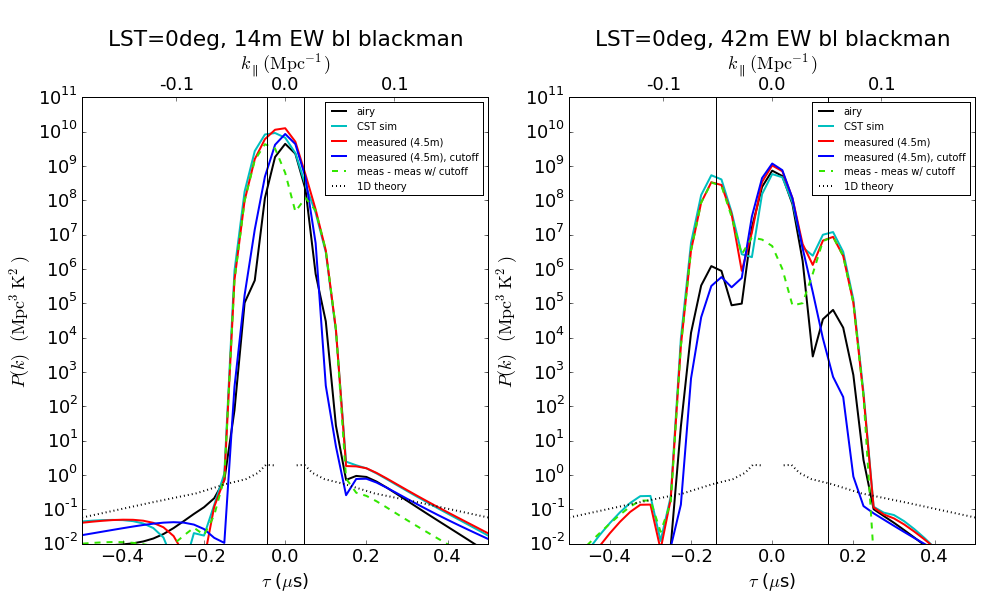
\includegraphics[width=5.5in]{LST0deg_14m_42m_EWbaselinesblackman.png}
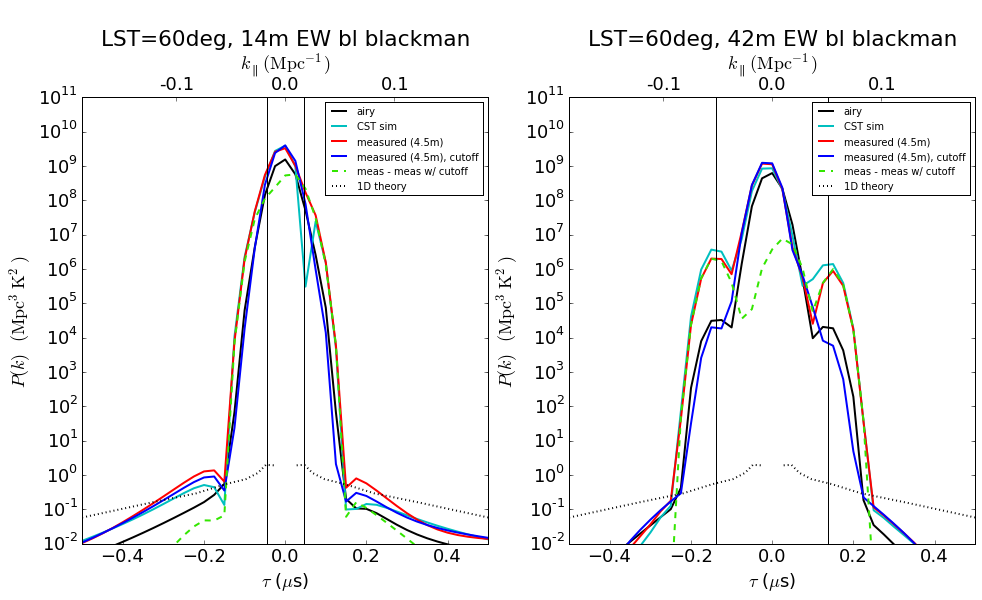
\includegraphics[width=5.5in]{LST60deg_14m_42m_EWbaselinesblackman.png}
\caption{aeuaoeuaoeu}
\label{fig:delayspec}
\end{figure*}

\begin{figure*}[h]
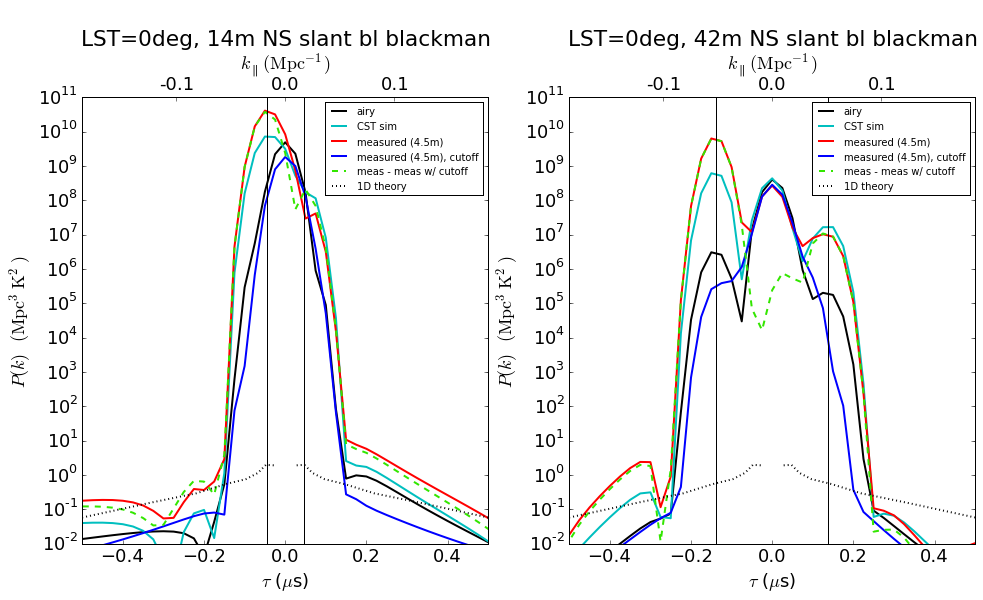
\includegraphics[width=5.5in]{LST0deg_14m_42m_NSslantbaselinesblackman.png}
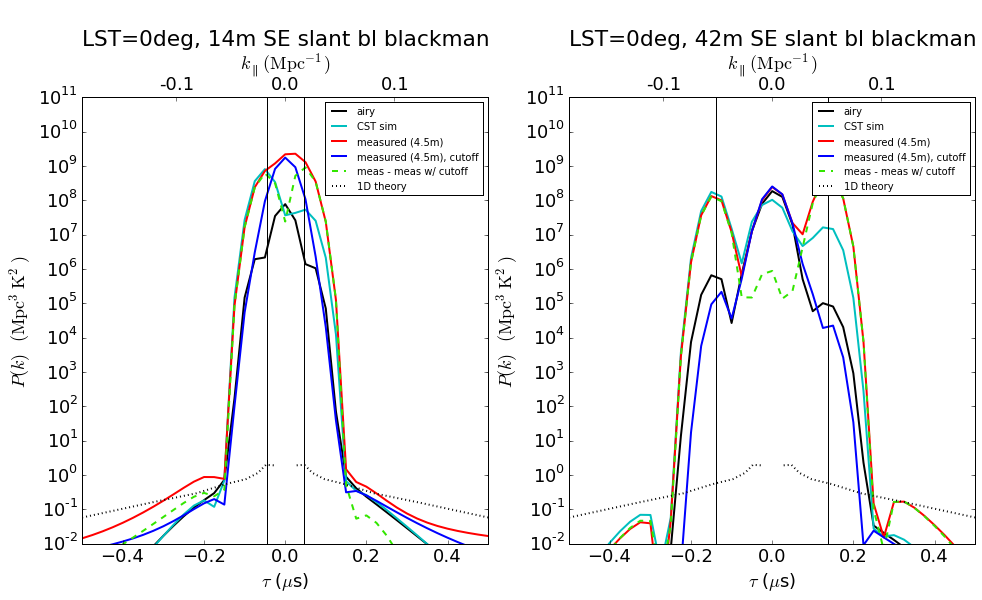
\includegraphics[width=5.5in]{LST0deg_14m_42m_SEslantbaselinesblackman.png}
\caption{aeuaoeuaoeu}
\label{fig:delayspec2}
\end{figure*}


\subsection{Foreground Residuals}
the accuracy of beam modeling affects the science performance in additional ways ranging from missubtraction to imperfect foreground subtraction (Neben et al. 2015b submitted). The impact of beam mismodeling on science performance is left as future work. 




\section{Discussion}

As expected, the Airy patter has the largest collecting area

the beam might be narrower simply because more dish is illuminated, but not necessarily a good thing, because we want more taper at the edge


comment on how this expt is still a work in progress









%% The reference list follows the main body and any appendices.
%% Use LaTeX's thebibliography environment to mark up your reference list.
%% Note \begin{thebibliography} is followed by an empty set of
%% curly braces.  If you forget this, LaTeX will generate the error
%% "Perhaps a missing \item?".
%%
%% thebibliography produces citations in the text using \bibitem-\cite
%% cross-referencing. Each reference is preceded by a
%% \bibitem command that defines in curly braces the KEY that corresponds
%% to the KEY in the \cite commands (see the first section above).
%% Make sure that you provide a unique KEY for every \bibitem or else the
%% paper will not LaTeX. The square brackets should contain
%% the citation text that LaTeX will insert in
%% place of the \cite commands.

%% We have used macros to produce journal name abbreviations.
%% AASTeX provides a number of these for the more frequently-cited journals.
%% See the Author Guide for a list of them.

%% Note that the style of the \bibitem labels (in []) is slightly
%% different from previous examples.  The natbib system solves a host
%% of citation expression problems, but it is necessary to clearly
%% delimit the year from the author name used in the citation.
%% See the natbib documentation for more details and options.

\bibliography{DishBeamMeasurementsMemo}


\end{document}
-